\documentclass[11pt,twoside]{article}
\addtolength{\textwidth}{0.5in}
\usepackage{epsfig,amsfonts,color}
\usepackage{amsmath}
\bibliographystyle{plain}
\usepackage{amssymb, palatino, geometry,url}
\usepackage{algorithmic}
\usepackage[noresetcount,lined,boxed]{algorithm2e} % ... for algorithms
\usepackage[colorlinks=true,linkcolor=blue,citecolor=blue,urlcolor=blue]{hyperref}
\geometry{letterpaper,
          left       = 0.9in,
          right      = 0.9in,
          top        = 0.9in,
          bottom     = 0.9in}
\linespread{1.2}

\usepackage{fancyhdr}
\usepackage{enumerate}
\usepackage{float}
\usepackage{subcaption}
\usepackage{graphicx}
\usepackage{caption}
\newcommand{\twopart}[4]
{
	\left\{
		\begin{array}{ll}
			#1 & \mbox{ } {\textrm{#2}} \\
			#3 & \mbox{ } {\textrm{#4}}
		\end{array}
	\right.
}

\newcommand{\N}{\mathbb{N}}
\newcommand{\Z}{\mathbb{Z}}
\newcommand{\Q}{\mathbb{Q}}
\newcommand{\R}{\mathbb{R}}
\usepackage{lineno}
%\linenumbers

\begin{document}

\title{Analysis of Multi-Scale Energy Markets using Stochatic Optimization Techniques}

\author{\textbf{\textit{ISyE 719 Course Project}}\\ \\Apoorva Sampat and Ranjeet Kumar\\
 {\small Department of Chemical and Biological Engineering}\\
 {\small \;University of Wisconsin, 1415 Engineering Dr, Madison, WI 53706, USA}}
\date{}
\maketitle

\begin{abstract}
Electricity markets operate at multiple timescales (from hours to milliseconds) to ensure that supply and demands are matched in real time. These markets involve uncertainties because future electricity prices and demands are unknown at the time of decision-making, e.g. energy sale and purchase commitments by generators. We use stochastic programming techniques to study flexibility and economic opportunities provided by a battery in these markets, namely day-ahead (1-hour timescale) and real-time (5-minute timescale) markets. In this work we consider uncertainty only in electricity loads and determine optimal participation strategies using methods like receding horizon scheme, dual dynamic programming and *fullproblem (scenario sampling)*. We also determine bounds on expected policy costs by using perfect information and two-stage approximation (with restriction on states). We compare the costs of participation in exclusively in day-ahead market and both day-ahead and real-time markets. Our results show that market participation only in day-ahead energy markets can *significantly* reduce economic flexibility as compared to participating in both levels of markets.
\end{abstract}


\section{Introduction}
A diverse set of energy systems such as generators, batteries, wind turbines and flywheels can participate in electricity markets. This participation is governed by rules set by ISOs (Independent System Operators) such as California ISO, PJM (Pennsylvania-New Jersey-Maryland) Interconnection and Midcontinent ISO, under whose jurisdiction the market falls. The markets are structured at multiple time levels, namely day ahead (hourly market commitments) and real time markets (commitments ranging from minutes to seconds). In day-ahead markets the electricity is traded in intervals of 1 hour with the prices being constant in each interval of 1 hour and varying with intervals. Real time markets, on the other hand can have varying time scales depending on the ISO operating it. The frequency of energy price variation is different for day-ahead and real time markets (Figure \ref{eprices}). 
\begin{figure}[h!tp]
\centering
\begin{subfigure}[b]{0.32\textwidth} 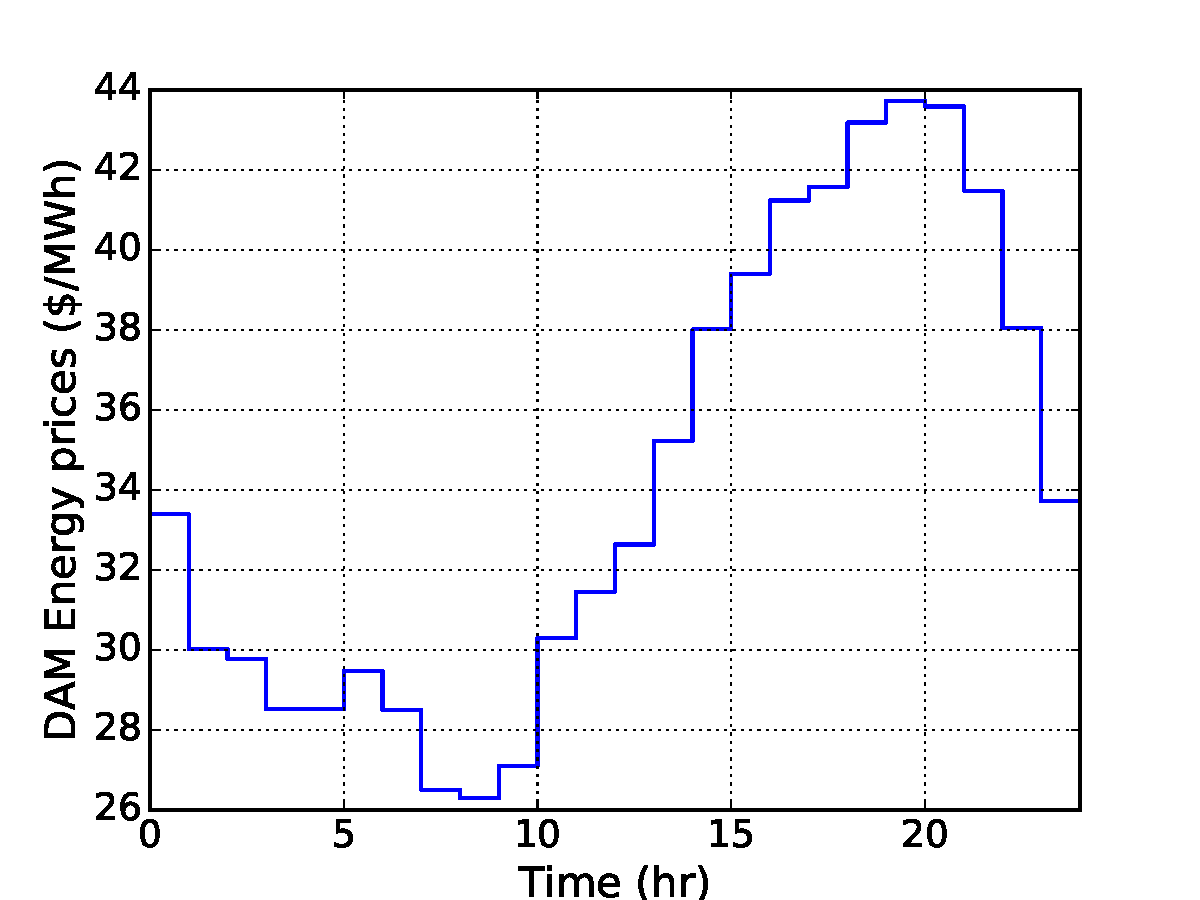
\includegraphics[width=\textwidth]{Figures/damprices.pdf} \caption{Day-ahead market}\label{damprices} \end{subfigure} \hfill
\begin{subfigure}[b]{0.32\textwidth} 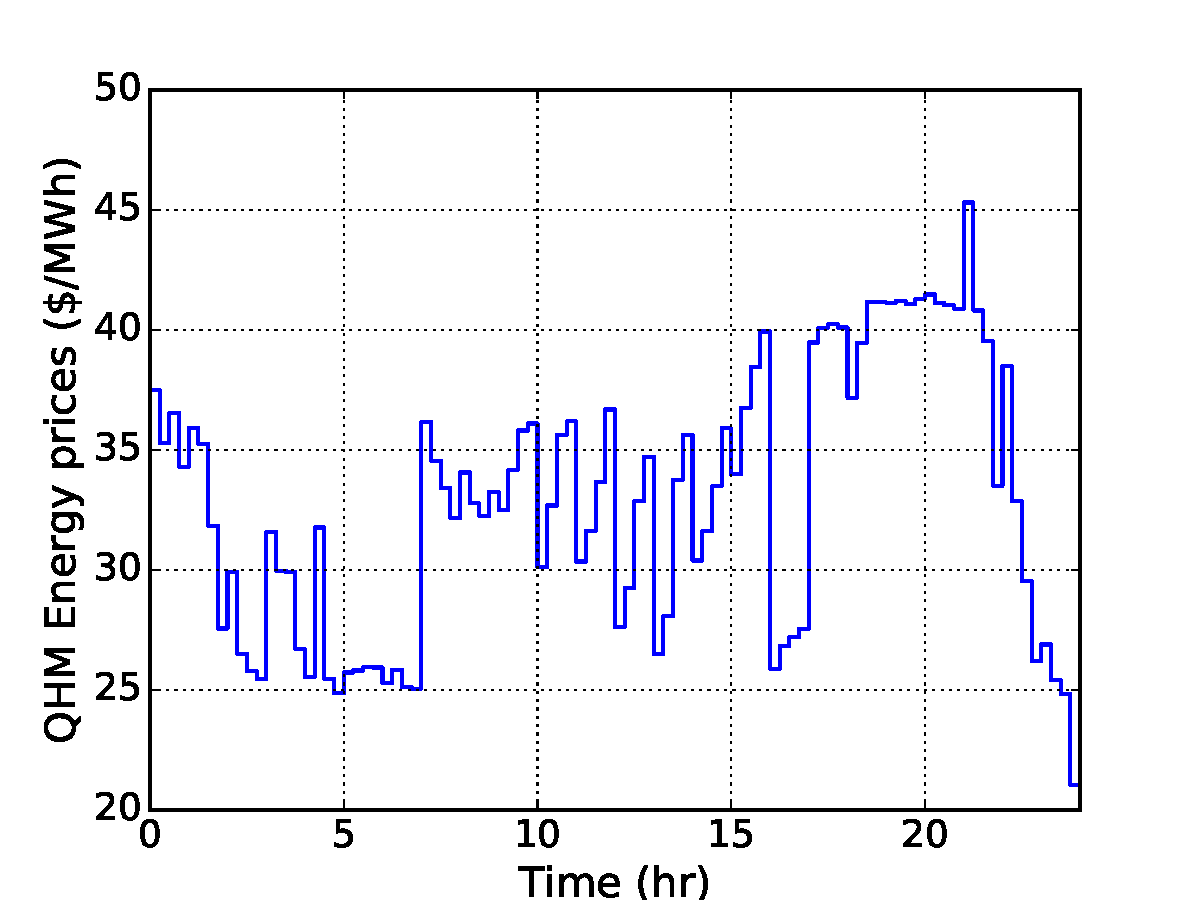
\includegraphics[width=\textwidth]{Figures/qhmprices.pdf} \caption{Quarter-hourly market}\label{qhmprices} \end{subfigure} \hfill
\begin{subfigure}[b]{0.32\textwidth} 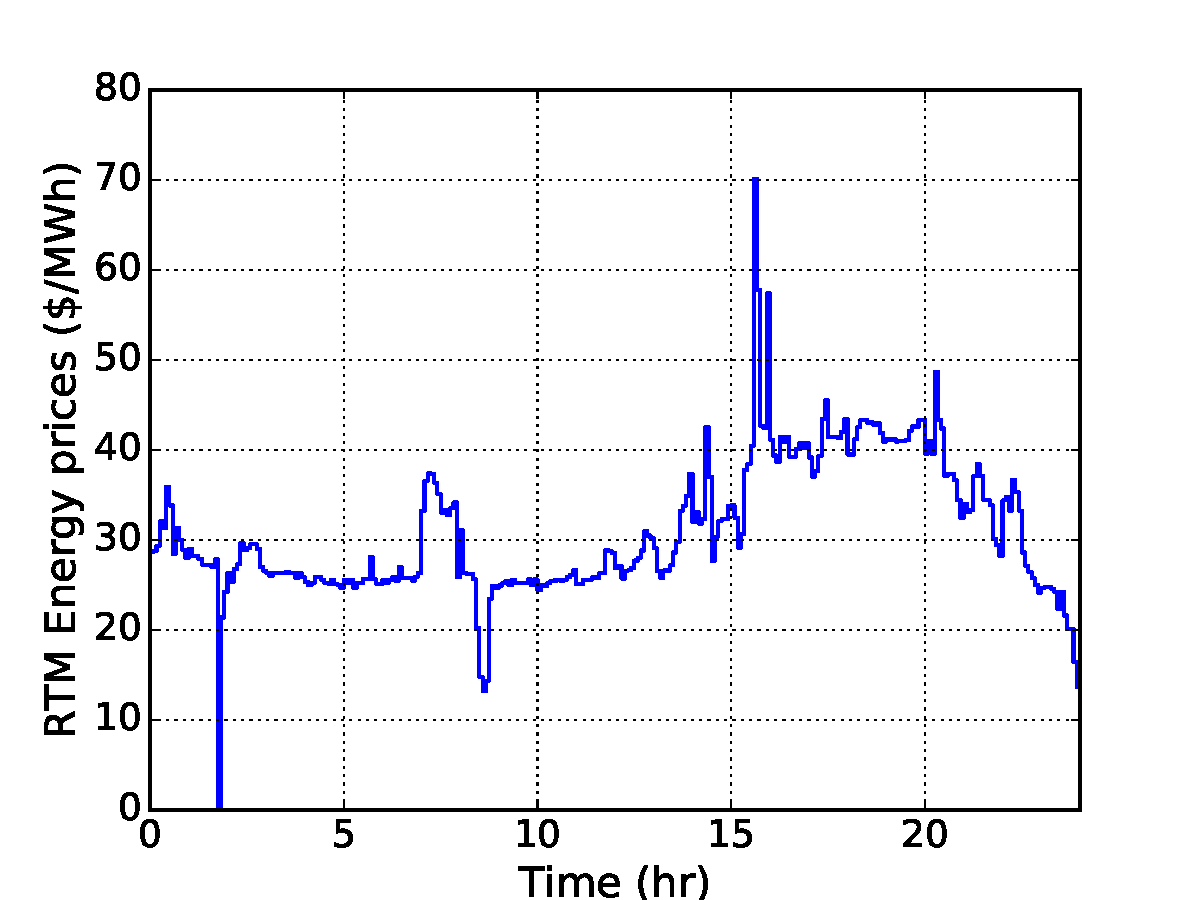
\includegraphics[width=\textwidth]{Figures/rtmprices.pdf} \caption{Real-time market}\label{rtmprices}\end{subfigure} \hfill
\caption{Energy prices for one day in the markets in California}\label{eprices}
\end{figure}



Apart from price variations, the introduction of more renewable power sources in the grid such as wind and solar energy, there are greater variations and uncertainties in the net load as well. Since these sources depend on intermittent conditions such as weather, they introduce slow dynamics to the grid. Thus systems with faster dynamic responses such as battery and building systems are becoming increasingly important to balance these fluctuations and provide dynamic flexibility to the power grid. Also, factors such as transmission losses, generation cost and congestion affect the value of products (energy, regulation, spinning , non-spinning reserves) offered at different timescales. These fluctuations being inherently uncertain, determining the optimal participation policy requires analysis using stochastic optimization techniques.
\begin{itemize}
\item \textbf{Day-ahead market :}
The day-ahead market is made up of three market processes that run sequentially. First, the ISO runs a market power mitigation test. Bids that fail the test are revised to predetermined limits. Then the integrated forward market establishes the generation needed to meet forecast demand. And last, the residual unit commitment process designates additional power plants that will be needed for the next day and must be ready to generate electricity. Market prices set are based on bids.

A major component of the market is the full network model, which analyzes the active transmission and generation resources to find the least cost energy to serve demand. The model produces prices that show the cost of producing and delivering energy from individual nodes, or locations on the grid where transmission lines and generation interconnect.

Scheduling coordinators (SCs) are pre-qualified entities authorized to transact in the ISO market. The day-ahead market opens for bids and schedules seven days before and closes the day prior to the trade date. Results are published at 1:00 p.m.

\item \textbf{Real-time market :} 
The real-lime market is a spot market in which utilities can buy power to meet the last few increments of demand not covered in their day ahead schedules. It is also the market that secures energy reserves, held ready and available for ISO use if needed, and the energy needed to regulate transmission line stability.

The market opens at 1:00 p.m. prior to the trading day and closes 75 minutes before the start of the trading hour. The results are published about 45 minutes prior to the start of the trading hour. The real-time market system dispatches power plants every 15 and 5 minutes, although under certain grid conditions the ISO can dispatch for a single 1-minute interval.

\end{itemize}
\section{Problem Definition and Decision-Making Setting}\label{sec:setting}
We consider a rechargeable Li-ion battery with a building that is inter-connected to the power grid for providing electricity services. Electricity services imply that batteries can provide power to or draw power from the grid. In our current setting, we do not consider participation in regulation or other ancillary services. The operator of the power grid (ISO) compensates the battery-owners for the electricity services provided. The goal for the battery-owners is to maximize the revenues generated by providing services to the grid and at the same time meeting the load demands from building. Any unmet load demand from the building is penalized.\\
\begin{figure}[h!]
\begin{center}
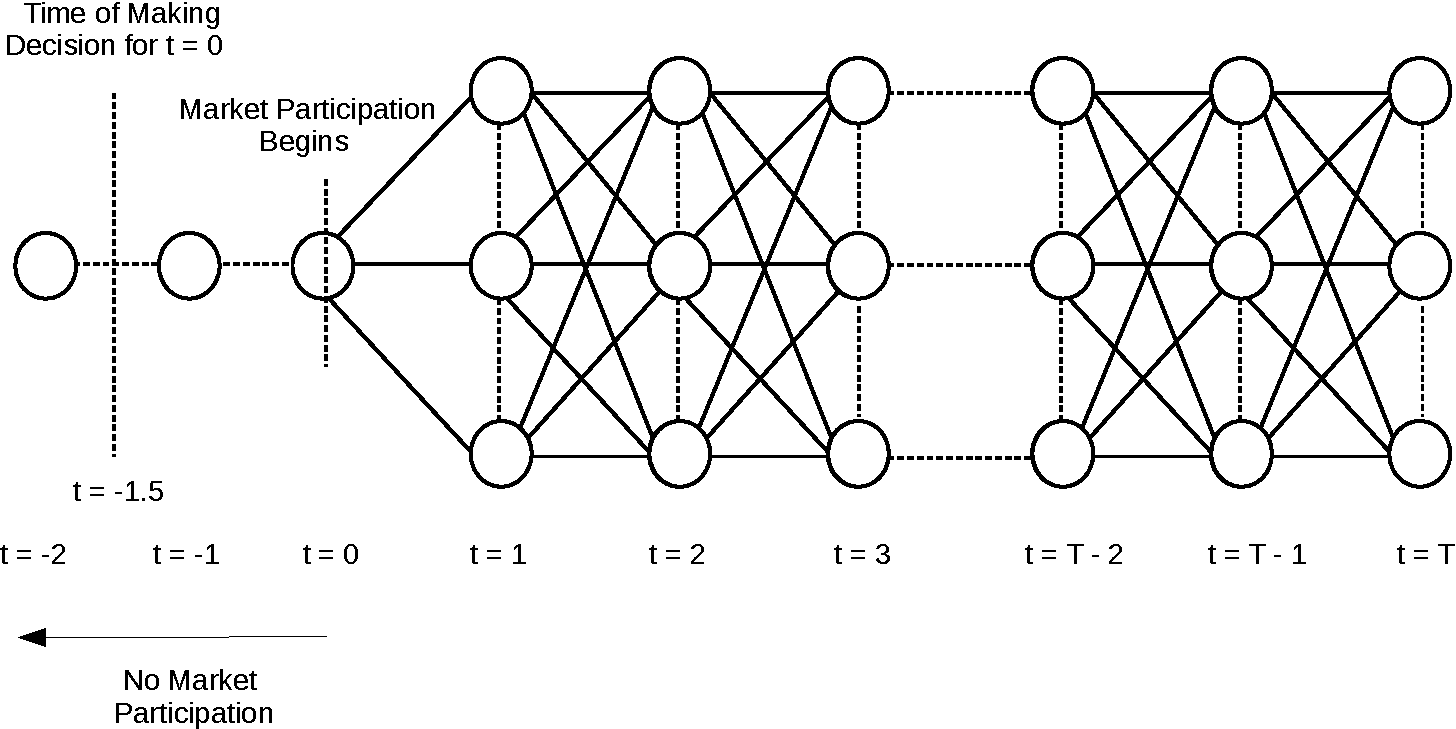
\includegraphics[width=4in]{Figures/scenario_tree-crop.pdf} \caption{Scenario tree at the beginning of market participation}\label{scenario_tree}\end{center}
\end{figure}

We divide an annual dataset for electricity loads (available over 5-minute intervals) into 52 subsets of weekly load profiles, i.e 2016 intervals of 5-minute each. This division of data helps in capturing the different load profiles over the weekdays and the weekend. We then use these 52 weekly profiles to generate sample scenarios for our computational experiments (Section \ref{sec:exp}). Since the loads are correlated between time intervals, we formulate a multivariate normal distribution for weekly loads using a mean vector and a covariance matrix. The mean vector (of size 2016 x 1) is the mean of the 52 datasets, but the covariance matrix (of size 2016 x 2016) calculated directly from the 52 datasets cannot be used, since its rank can at most be 52. So we use the Ledoit-Wolf Covariance Estimator \cite{ledoit2004well} (to tackle rank deficiency) for estimating a full rank covariance matrix. We generate 50 samples of load profiles (Figure \ref{fig:loads_scenarios}) for a week using the mean and covariance matrix obtained. 
\begin{figure}[h!]
\begin{center}
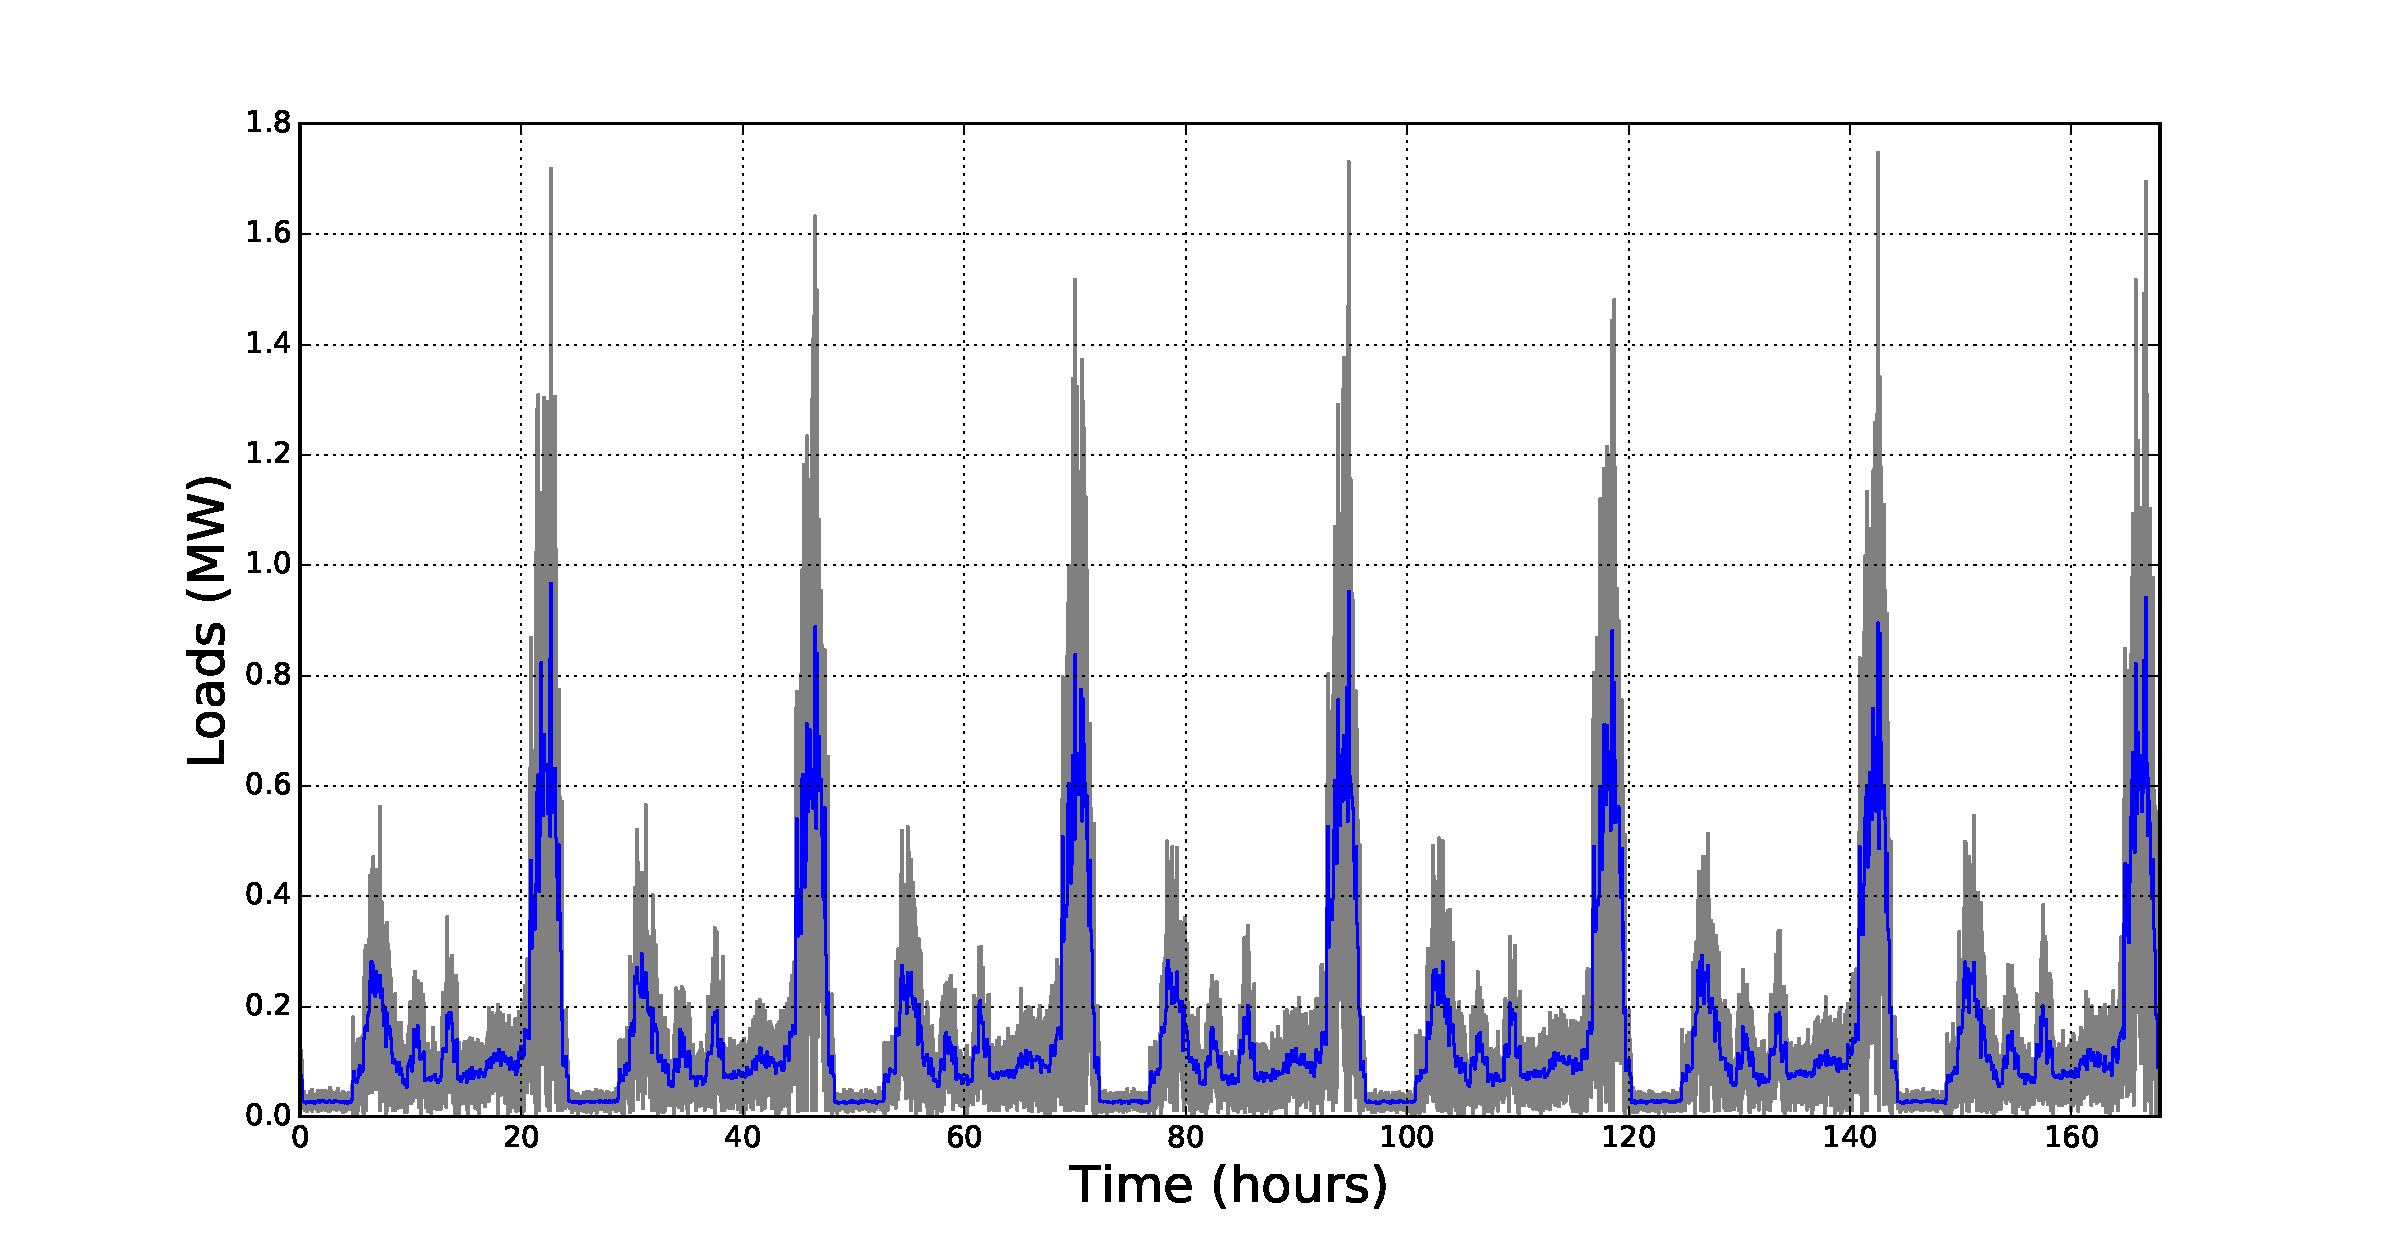
\includegraphics[width=4in]{Figures/Plots/fullproblem_stoch/loads_scenarios.pdf} \caption{Load scenarios for a week}\label{fig:loads_scenarios}\end{center}
\end{figure}



Cosidering the price data for a full year to be known (deterministic) we can solve the optimization problem to maximize the annual revenues by operating a battery in the power grid for the whole year. In this work, we aim to solve this deterministic optimization problem with two approaches:
\begin{enumerate}
\item Simultaneous approach: In this approach, we formulate a single giant optimization problem for a full year and solve it to produce the optimal power and regulation capacities that the battery should operate with in each time interval in all the three markets. 
\item Rolling (1 day) horizon approach: In this approach, we formulate an optimization problem for a day and solve it to produce the optimal power and regulation capacities for that day, then take the solutions at the end time-point of that day as the initial point for the next day, then formulate the optimization problem for the next day with those initial values and solve for the second day and sequentially we solve for the 365 days. It is called rolling horizon because in this approach we consider a horizon of 1 day and keep shifting the horizon to to the next day after solving the current day.
\end{enumerate}

At the end, we will compare the two solutions and investigate the advantages and disadvantages of the two approaches.

Understanding the economic incentives provided by generation and load flexibility requires of careful consideration of wholesale electricity market structures and diverse products. Figure \ref{fig:market_control_structure} shows the multiscale control structure currently used to balance the power grid. Resources can participate by buying/selling electrical energy and/or providing ancillary services (regulation, reserves). Figure \ref{fig:energy_AS_prices} shows time-varying prices from the California Independent System Operator (CAISO) for three consecutive days. Energy is transacted at three timescales: in the integrated forward market (day-ahead market with 1-hour intervals), in the fifteen minute market, and through the real-time dispatch process (5-minute intervals). Table \ref{tab:caiso_products} lists the different products transacted at each timescale. Histograms for energy prices at different markets are presented in Figure \ref{fig:CAISO_prices2}. As can be seen, prices are less volatile in the day-ahead market and the average price is higher. In the real-time market (FMM, RTD) prices are frequently negative and occasionally exceed \$150/MWh. Energy systems with fast dynamics (e.g., flywheels, batteries) can exploit these fast price fluctuations.

In the U.S., generators/loads provide the hierarchical market structure with addition flexibility via \emph{regulation} and \emph{reserve} ancillary service products. 

\section{Optimization Model for Battery Systems}\label{sec:model}
\subsection{Perfect Information Setting}
The optimization model for each day can be formulated as follows:\\
\paragraph{Sets:}
\begin{subequations}
\begin{align}
R := \{1,..,n_r\},\,\; D :=  \{1,..,n_d\}
\end{align}
\end{subequations}
Here, R is the set of time indices for the real-time subintervals within each quarter-hour interval, so $n_r=12$, so D is the set of time indices for the hourly intervals within each day, so $n_d=24$.\\
\paragraph{Indices:}
\begin{subequations}
\begin{align}
i \in R, \;\; k \in D
\end{align}
\end{subequations}
\paragraph{Constraints for each day in the model:}
\begin{subequations}
\begin{align}
&P_{{net}_{i,k}} = P_{i} + P_{i,k} + L_{i,k}\\
\end{align}
\label{eq:Pnet}
\end{subequations}
\begin{subequations}
\begin{align}
&E_{1,1} = E_{0} - P_{{net}_{i,k}}\Delta t_r\\
\end{align}
\label{eq:eq1}
\end{subequations}
\vspace{-0.45in}
\begin{subequations}
\begin{align}
E_{i,k} =&\; E_{i-1,k}- P_{{net}_{i,k}}\Delta t_r\\
E_{1,k} =&\; E_{n_r,k}- P_{{net}_{1,k}} \Delta t_r\\
\end{align}
\label{eq:eq2}
\end{subequations}
\vspace{-0.45in}
\begin{subequations}
\begin{align}
0 & \leq E_{i,j,k} \leq E_{max}\\
-P_{max} & \leq P_{i,k} \leq P_{max}\\
-P_{max} & \leq P_{k}\phantom{i,} \leq P_{max}\\
\end{align}
\label{eq:eq4}
\end{subequations}\vspace{-0.45in}
\begin{subequations}
\begin{align}
Rev_E =& \sum_{i \in R} \sum_{k \in D} \Delta t_r(\pi^E_{i,k}P_{i,k}) + \sum_{k \in D}\Delta t_d(\pi^E_{k}P_{k})\\
\end{align}
\label{eq5}
\end{subequations}
Here, the decision variables are $E$, the energy of the battery at every time interval, $P$, the net power of the battery going to the power grid in the three markets, $R^U$, the regulation up capacities in the two levels of regulation markets, $R^D$, the regulation down capacities in the two levels of regulation markets and $Rev^E$ and $Rev^R$, the revenues from the energy and regulation markets respectively. The three subscripted indices in $P$, $R^U$ and $R^D$ variables mean that they are for the real-time market, the two subscripted indices in $P$, $R^U$ and $R^D$ variables mean that they are for the quarter-hourly market and the one subscripted index in $P$, $R^U$ and $R^D$ variables mean that they are for the day-ahead market. $\pi$'s are the prices which are known parameters in the model, the superscript on $\pi$ denotes the quantity which it is the price of and subscripts on $\pi$ denotes the level of market of which it is the price.

\subsection{Optimization Under Uncertainty}

\section{Computational Experiments}\label{sec:exp}
List of figures

\subsection{Full Problem}
In this case study, we sample 50 scenario paths (out of the $50^{168}$ possibilities) for a week's time period. We then construct a full model for for this week and use real price signals from 01/01/2015 to 01/07/2015 in California ISO \footnote{http://oasis.caiso.com/mrioasis/logon.do}. For every 1 hour interval in the model, we sample a scenario, and use the load data corresponding to that scenario for the 12 intervals (5 minutes each) in that hour. This helps to reduce the size of scenario tree (from $50^{168 \times 12}$ to $50^{168}$). We solve this model (with 50 sampled paths) 100 times to get a confidence interval on the expected revenue. We then compare this expected revenue (obtained by participating in both real time and day-ahead market) to the cases when the battery participates only in either real time or day-ahead market alone.
\begin{itemize}
\item Supplied and unmet load for a sample path
\item Prtm
\item Pdam
\item SOC 
\item Net discharge
\item revenue from energy : \$ 739.73, \\ from dam: 815.74 \\ from rtm:  -84.76 (loss) \\unmet cost: - 8.75   (i.e. buy from outside when prices are negative)
get's more flexibility to dam participation. 
\item only rtm: total revenue: \$ 70.03 , unmet = -9.10, profit from rtm market =  60.93
\item only dam: total revenue: \$ - 921.61, unmet cost = 76.93, profit edam = -844.68. (needs to buy energy to supply to battery) 
\end{itemize}
\begin{tabular}{|c|c|c|c|c|}
\hline 
Market Participated  & Total Revenue (\$) & Unmet Load Cost (\$) & DAM Revenue  (\$) & RTM Revenue (\$) \\ 
\hline 
DAM + RTM & 739.73 & -8.75 & 815.74 & -84.76 \\ 
\hline 
DAM & -921.61 & 76.93 & -844.68 & N/A \\ 
\hline 
RTM & 70.03 & -9.10 & N/A & 60.93 \\ 
\hline 
None & -10,293.23 & 10,293.23 & • & • \\ 
\hline 
\end{tabular} 


\begin{figure}[h!]
\begin{center}
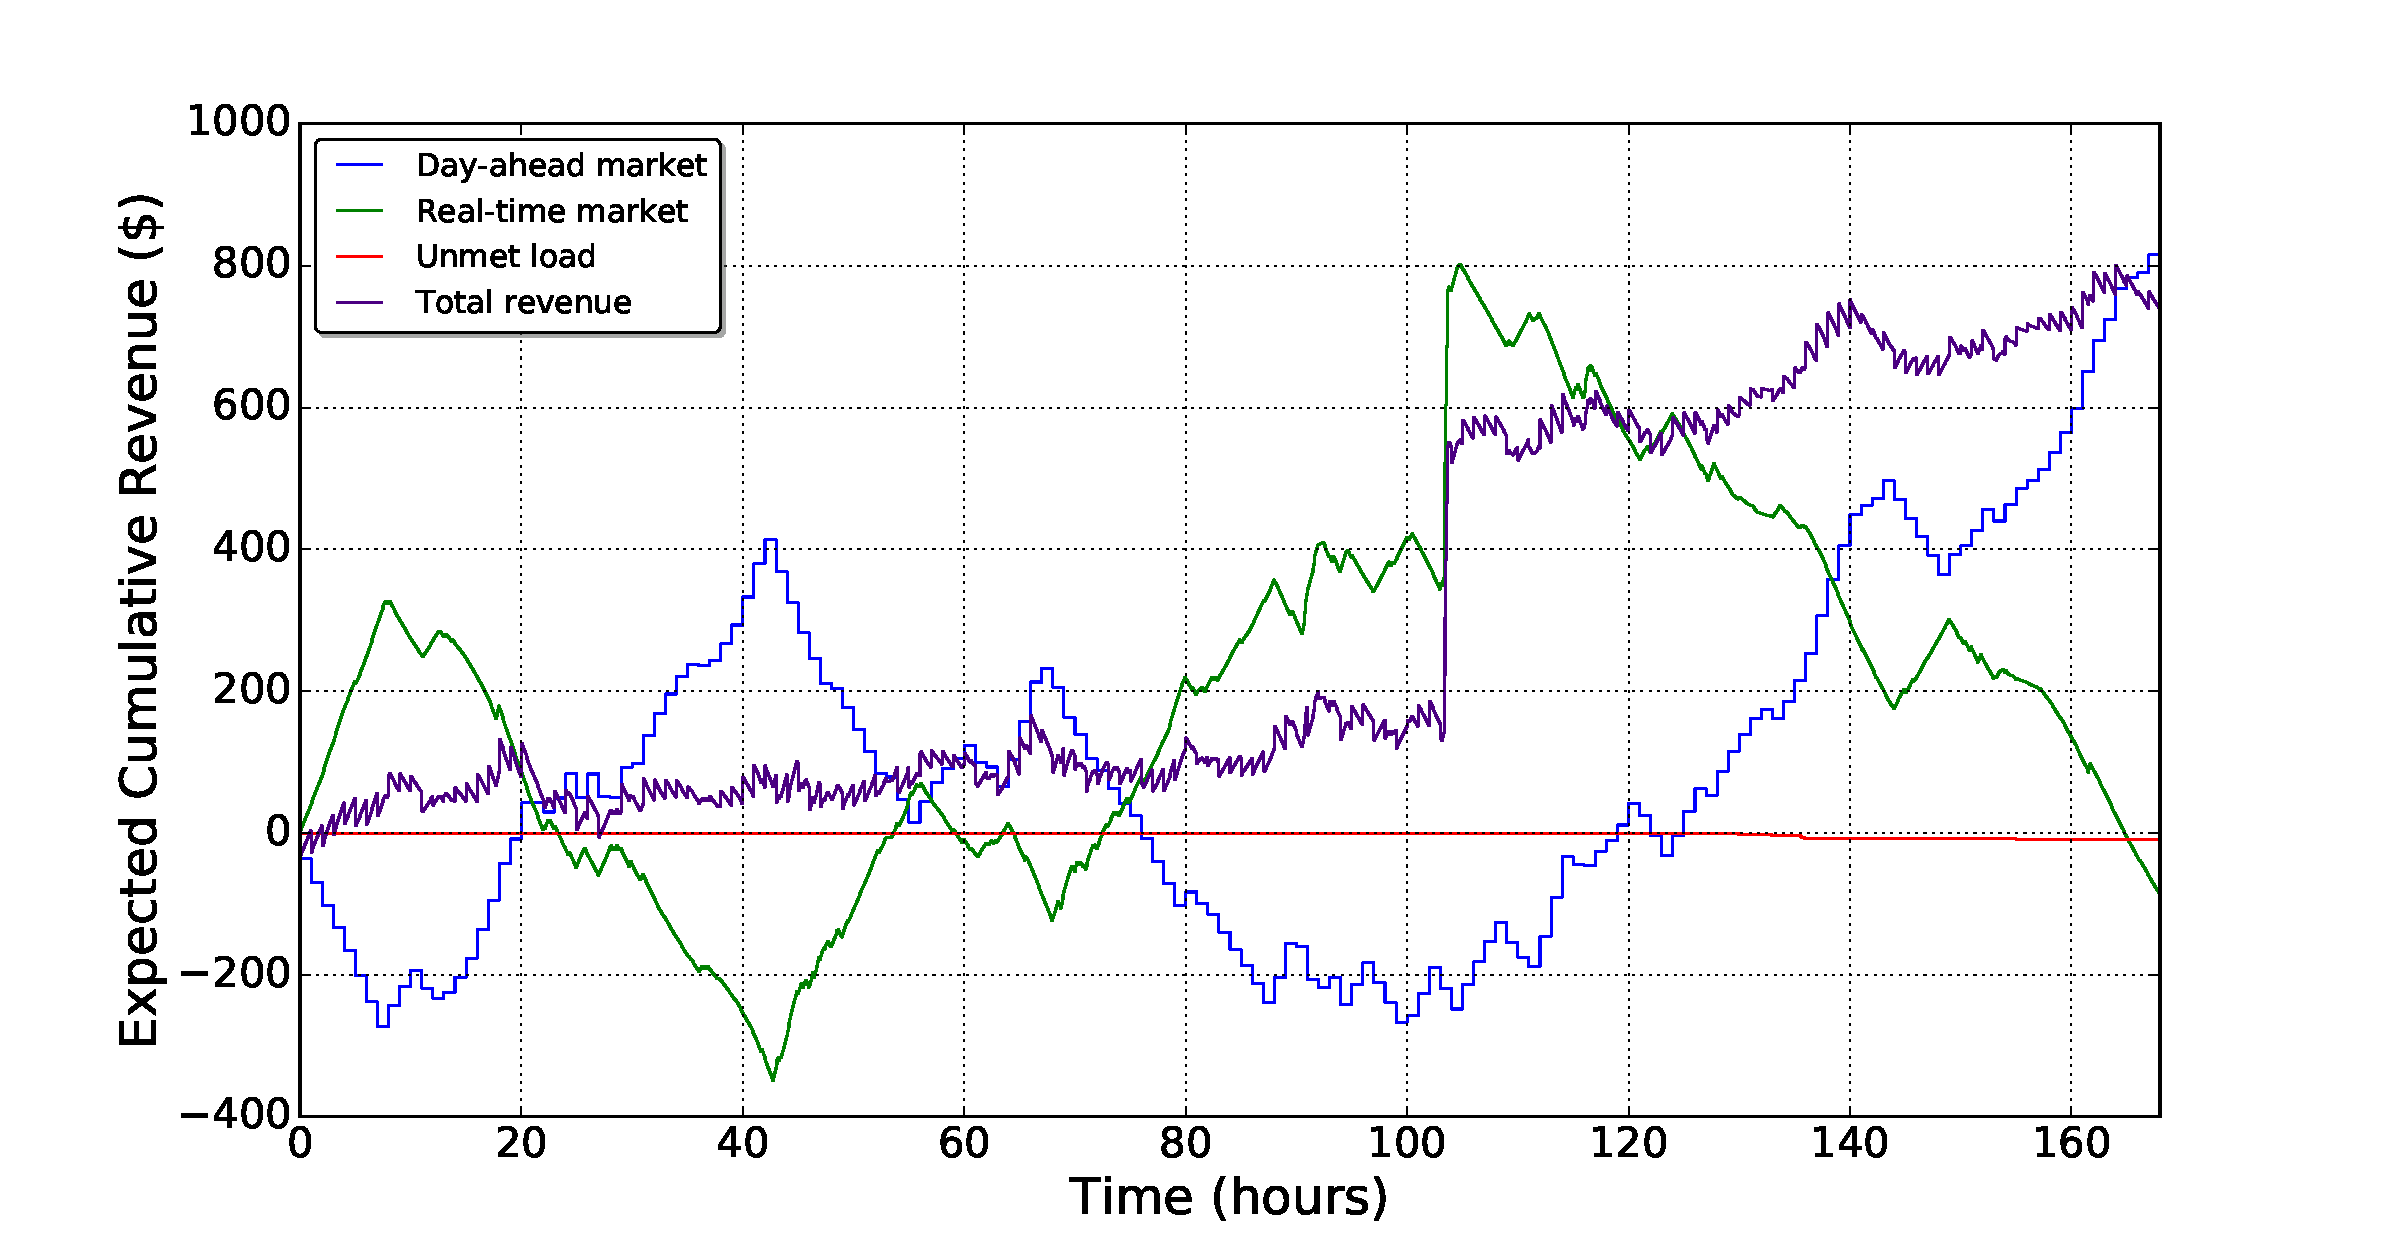
\includegraphics[width=4in]{Figures/Plots/fullproblem_stoch/cumulative_rev_fp_st.pdf} \caption{Trajectory of cumulative revenues}\label{cumulative_rev_fp_st}\end{center}
\end{figure}
\begin{figure}[h!]
\begin{center}
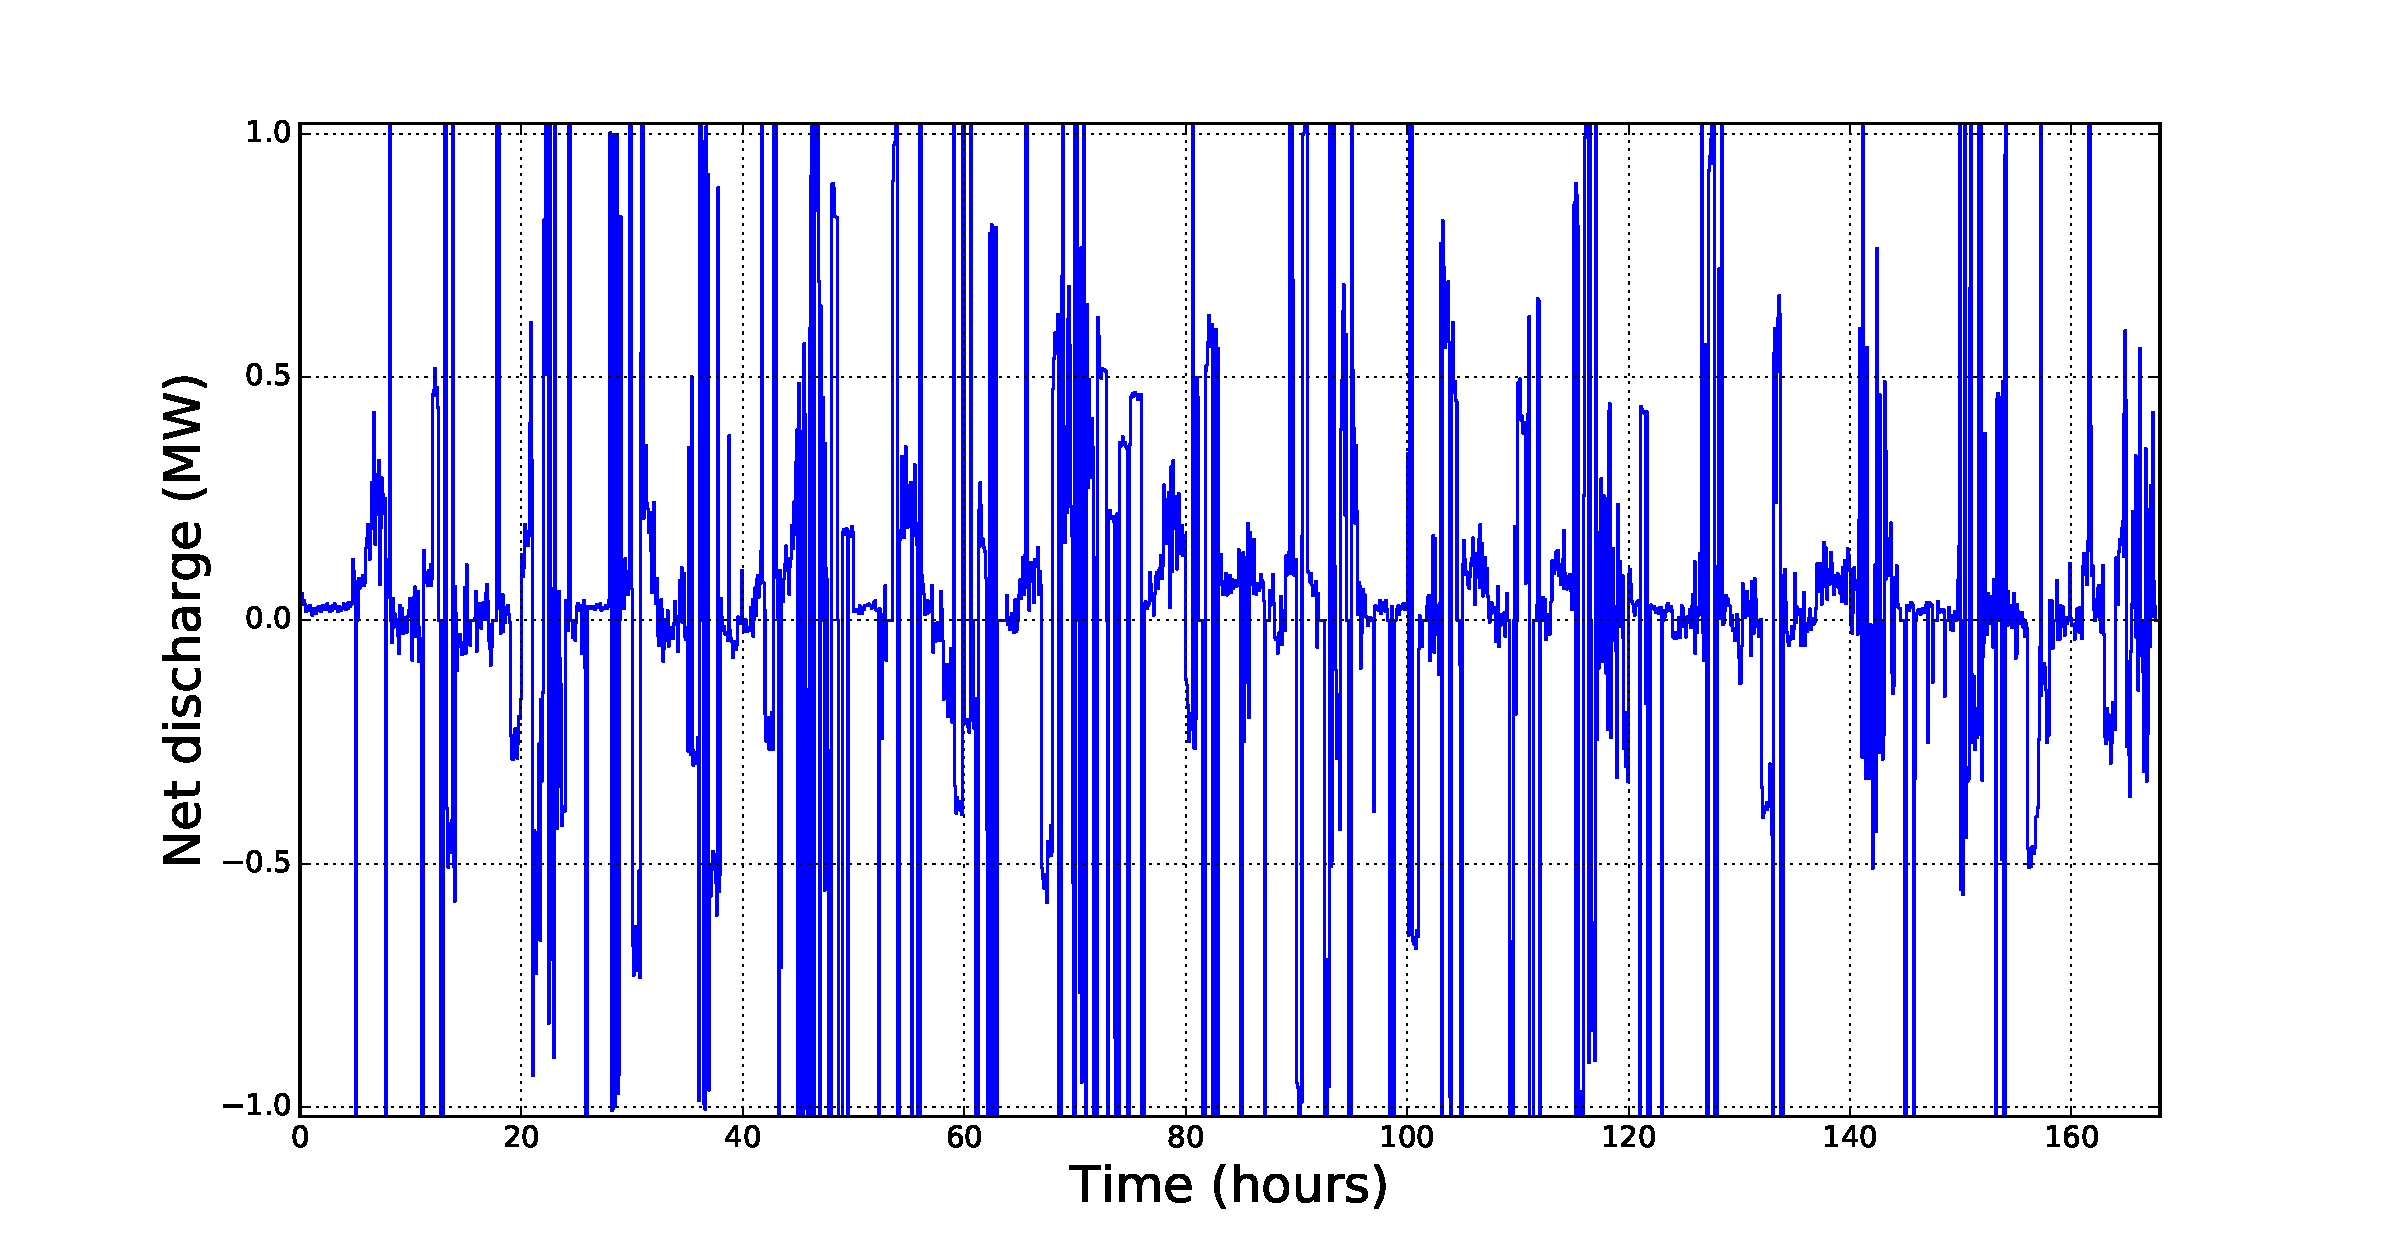
\includegraphics[width=4in]{Figures/Plots/fullproblem_stoch/netpower_fp_st.pdf} \caption{Net battery discharge}\label{netpower_fp_st}\end{center}
\end{figure}
\begin{figure}[h!]
\begin{center}
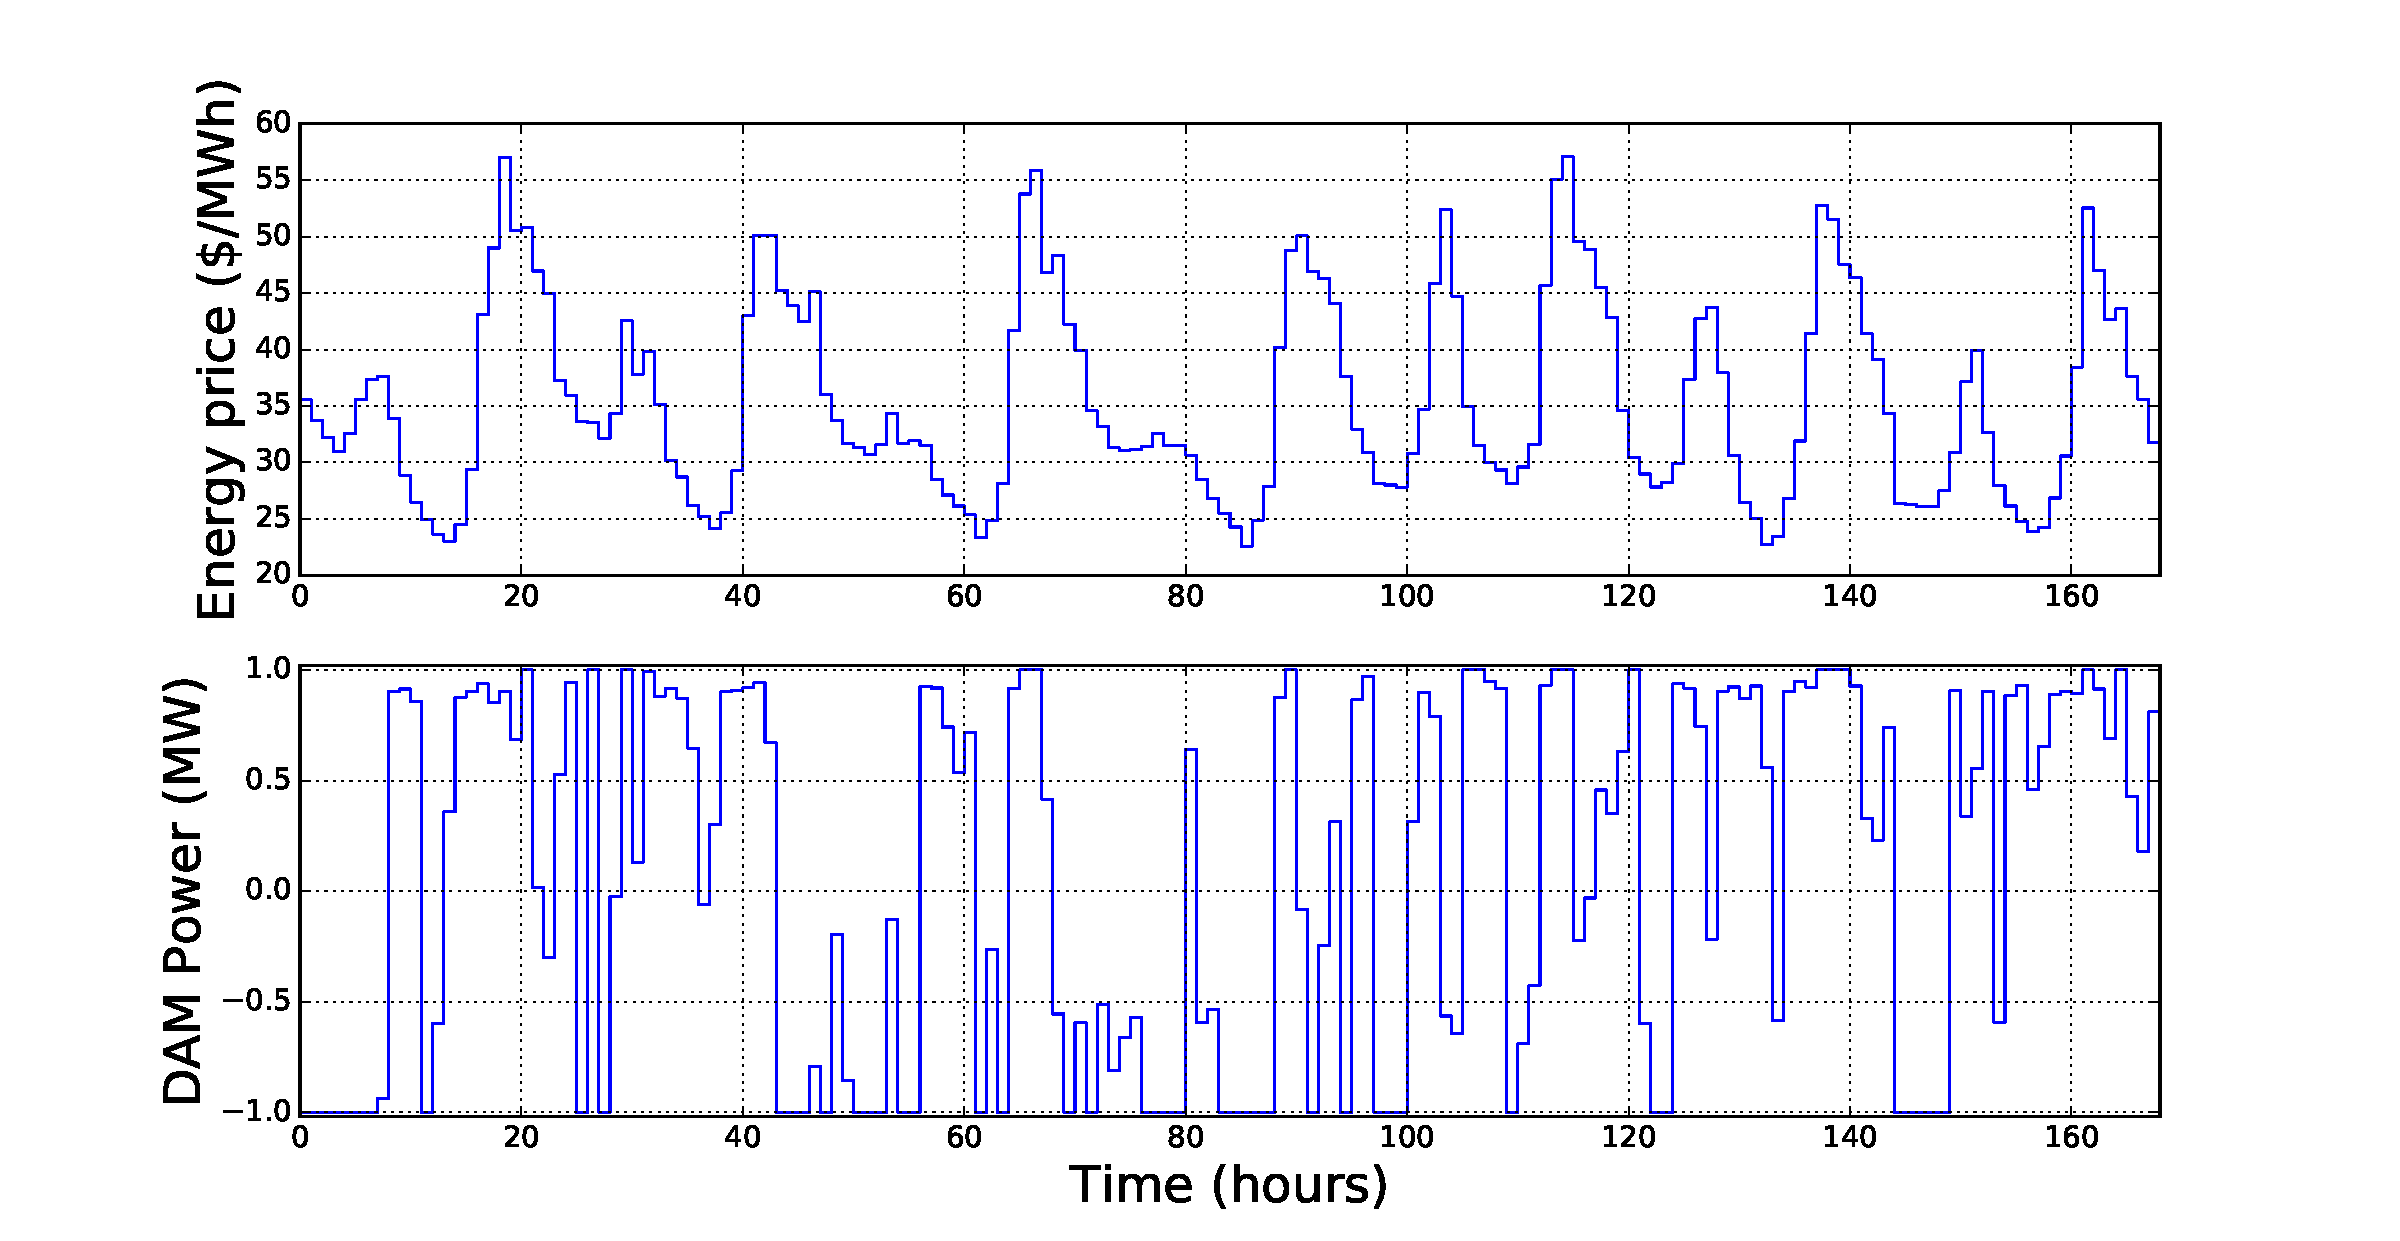
\includegraphics[width=4in]{Figures/Plots/fullproblem_stoch/Pdam_fp_st.pdf} \caption{Energy participation policy in day-ahead market}\label{Pdam_fp_st}\end{center}
\end{figure}
\begin{figure}[h!]
\begin{center}
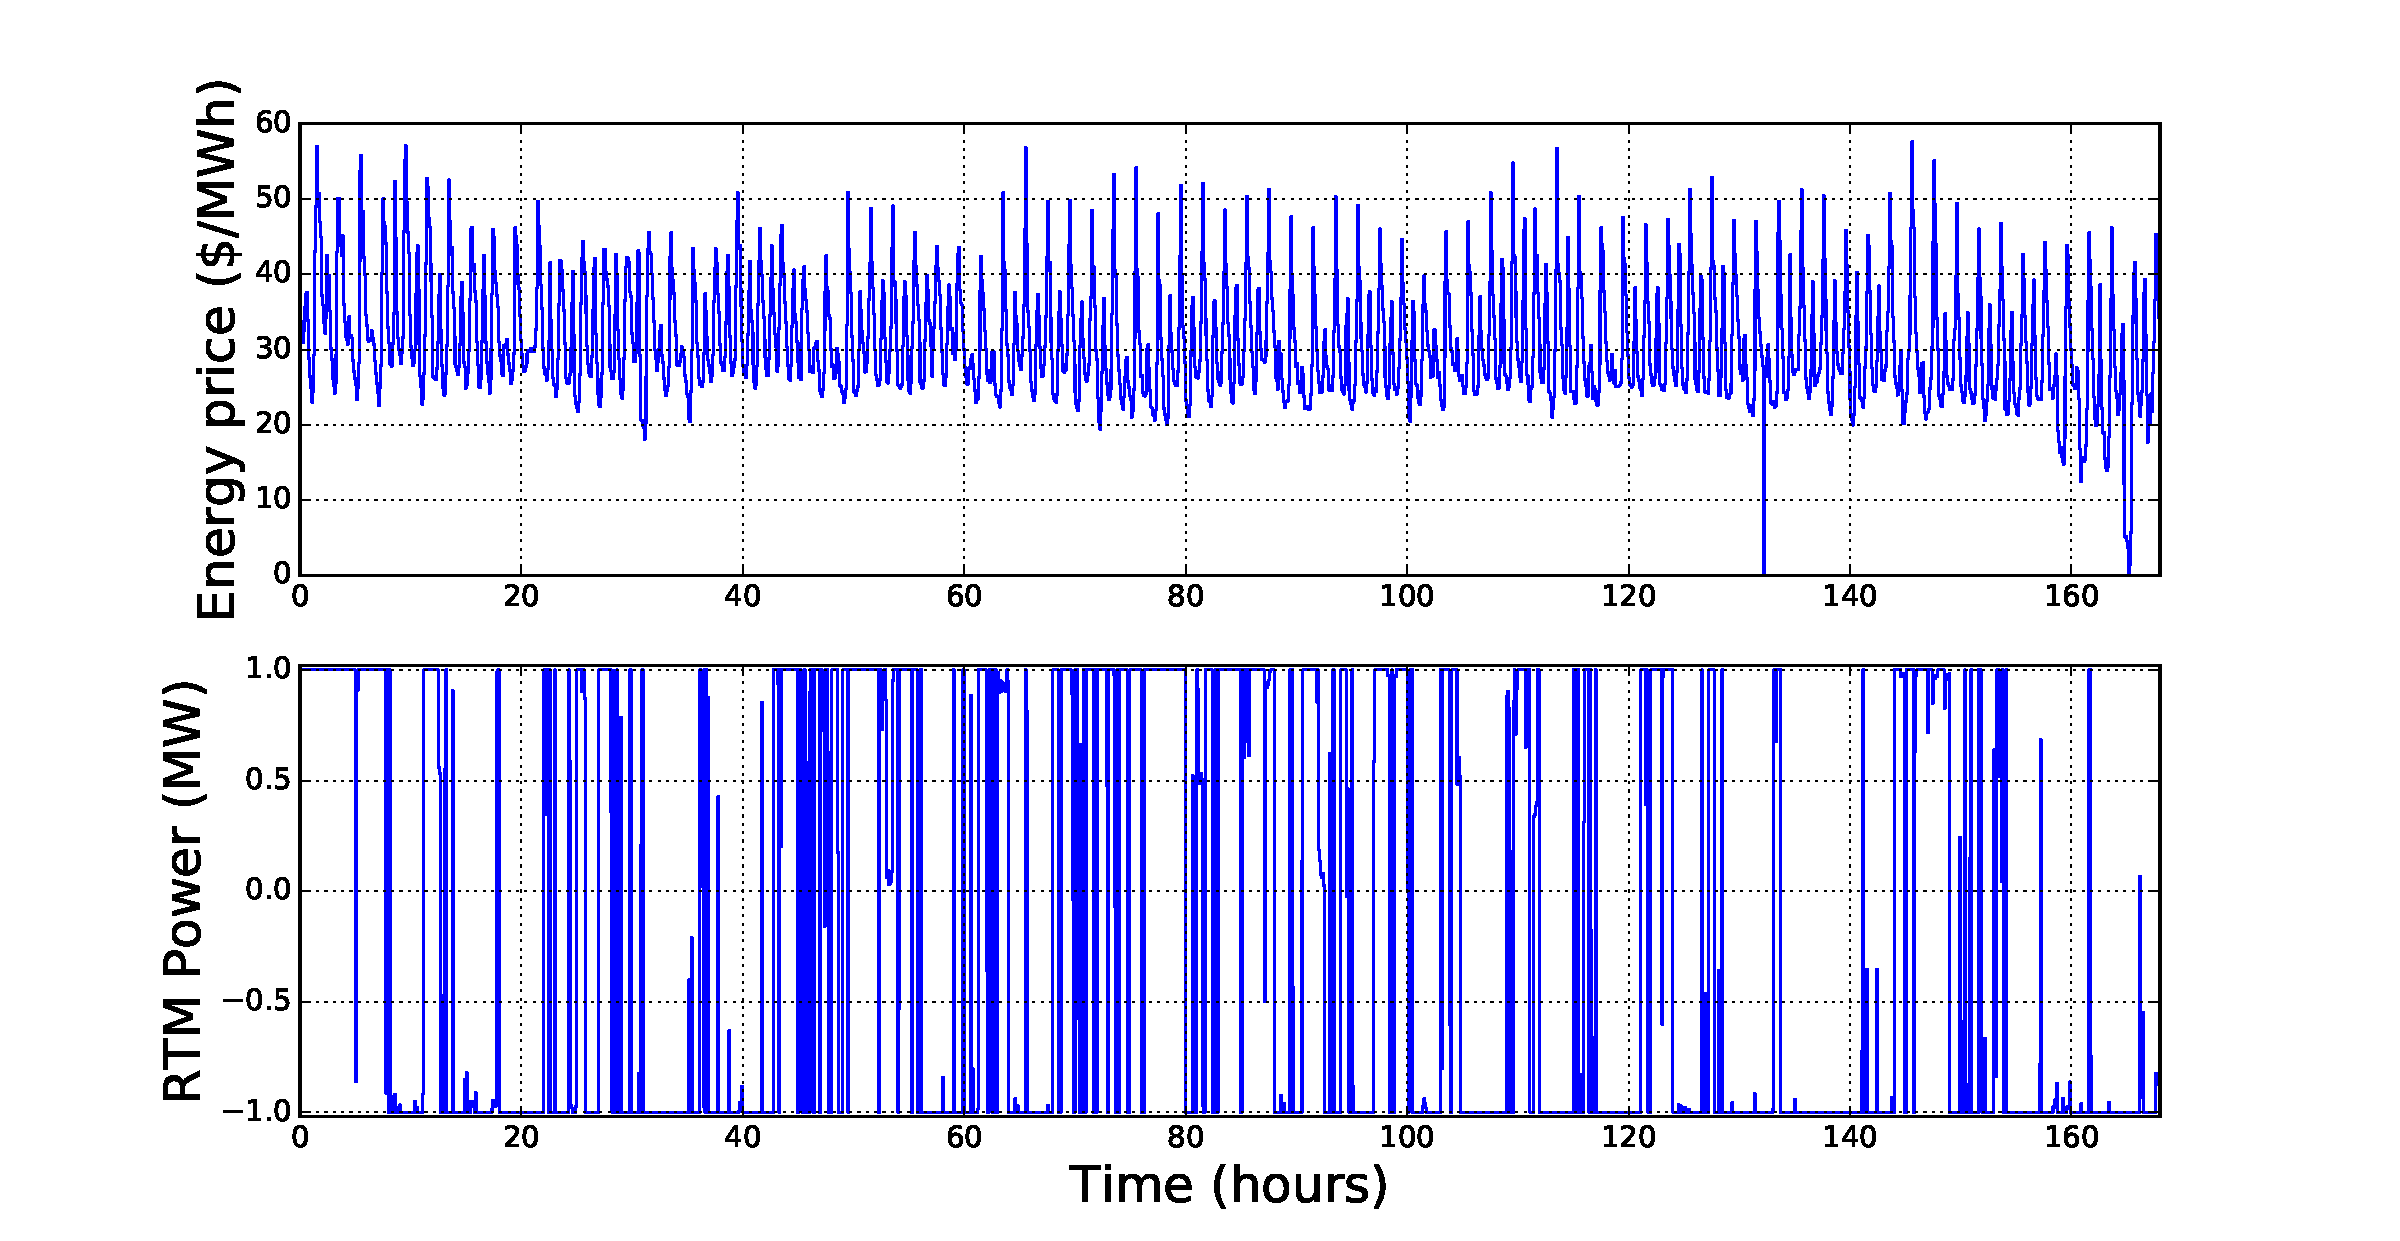
\includegraphics[width=4in]{Figures/Plots/fullproblem_stoch/Prtm_fp_st.pdf} \caption{Energy participation policy in real-time market}\label{Prtm_fp_st}\end{center}
\end{figure}
\begin{figure}[h!]
\begin{center}
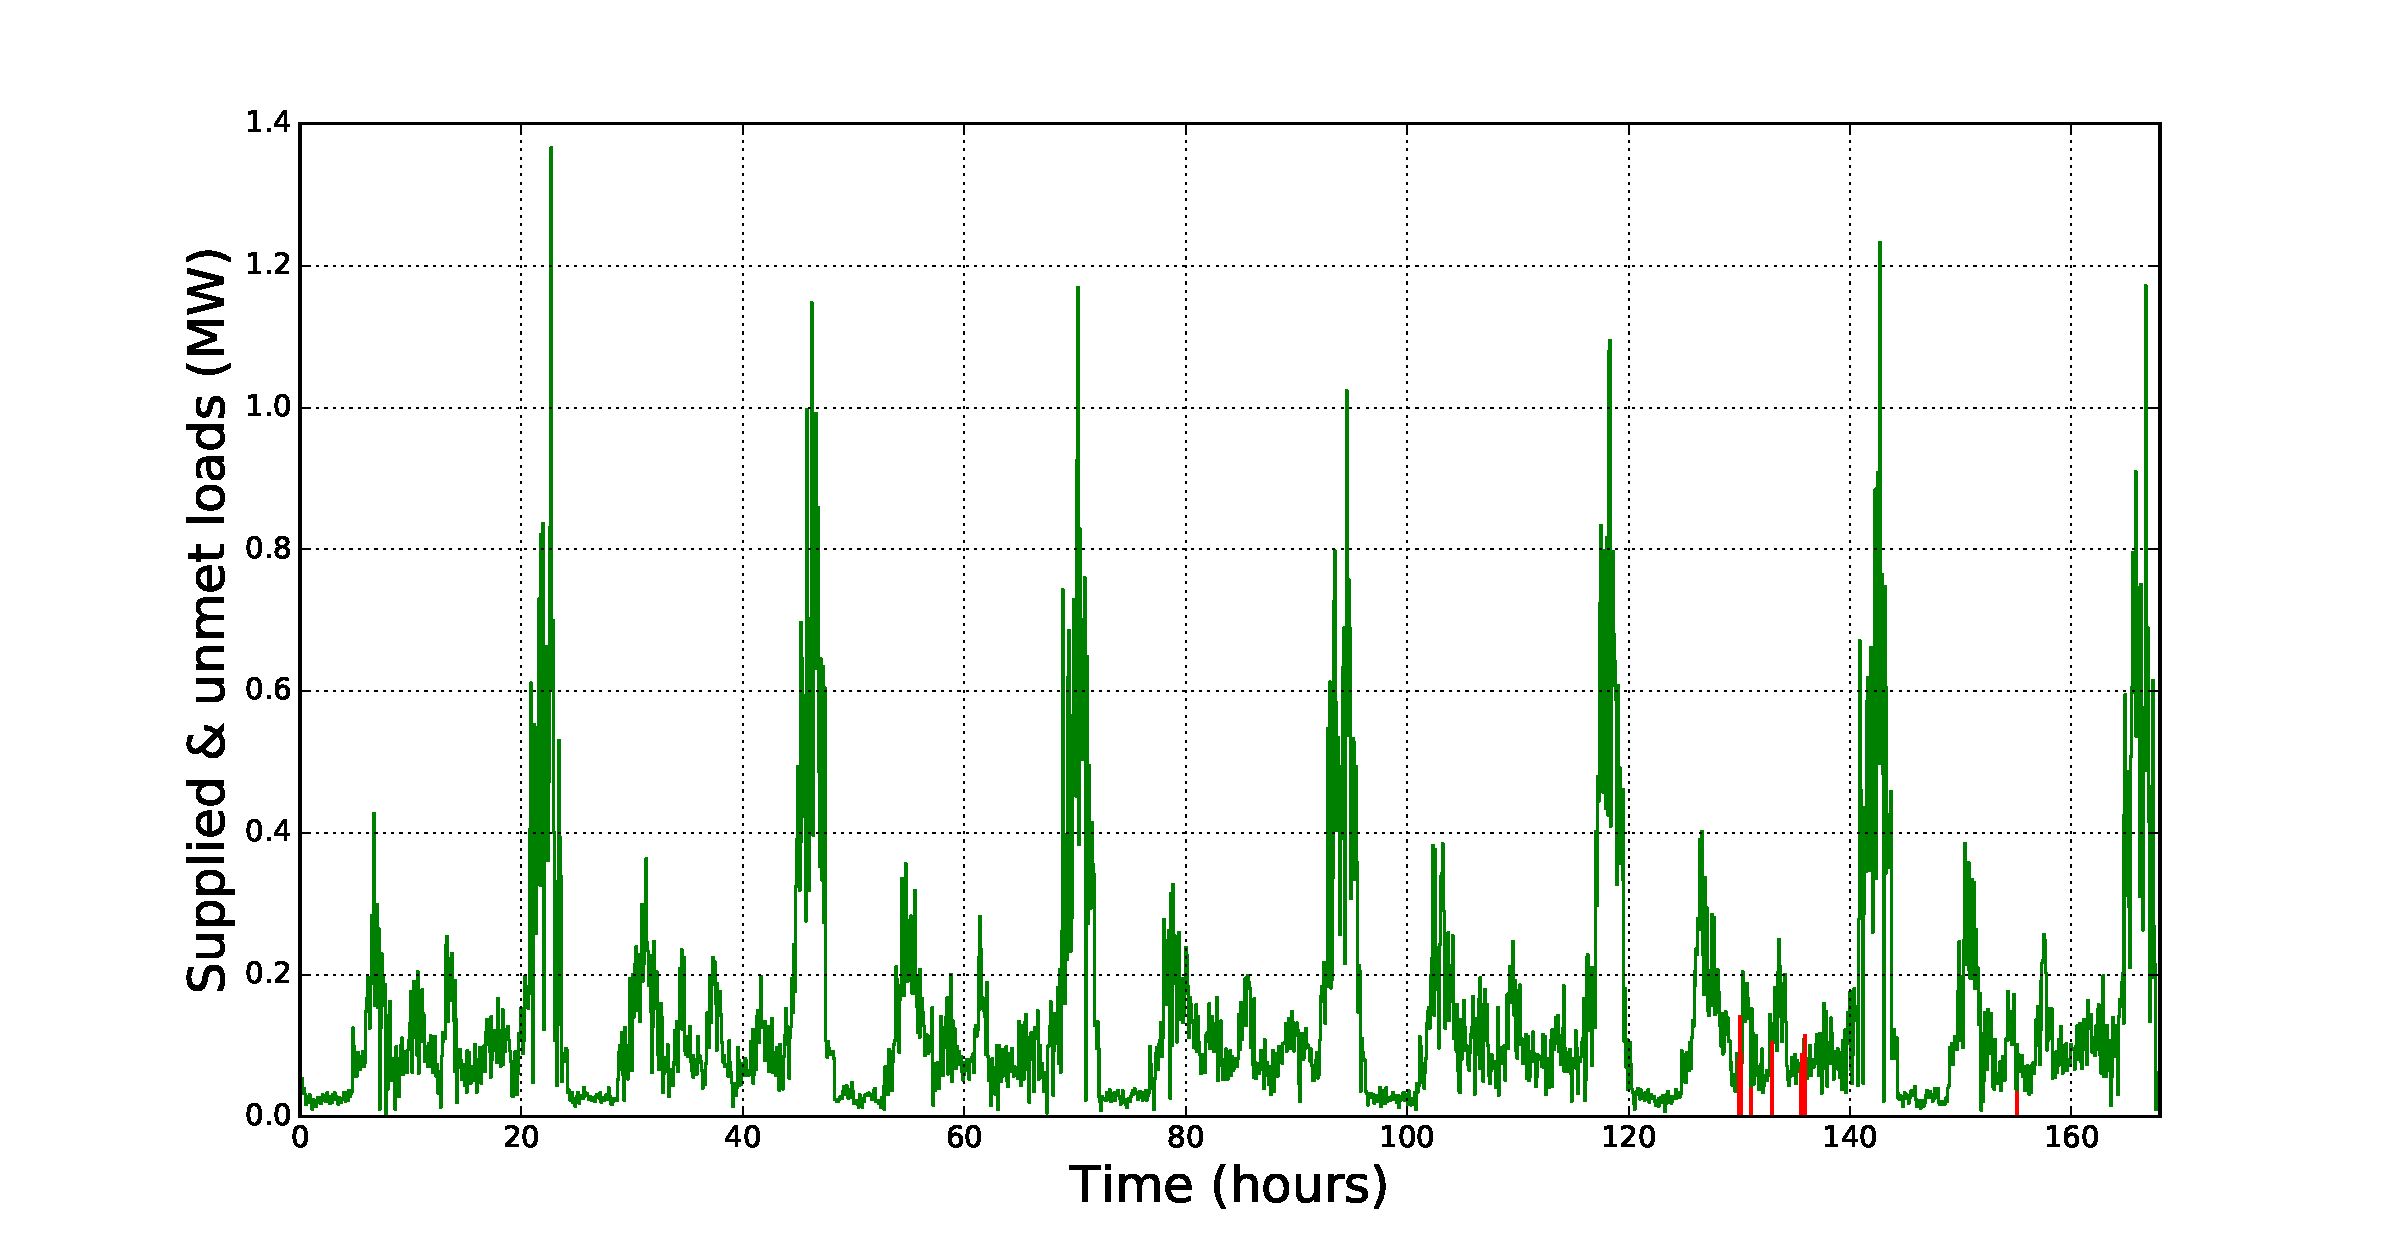
\includegraphics[width=4in]
{Figures/Plots/fullproblem_stoch/supp_unmet_fp_st.pdf} \caption{Power supplied to building and unmet load}\label{supp_unmet_fp_st}\end{center}
\end{figure}
\begin{figure}[h!]
\begin{center}
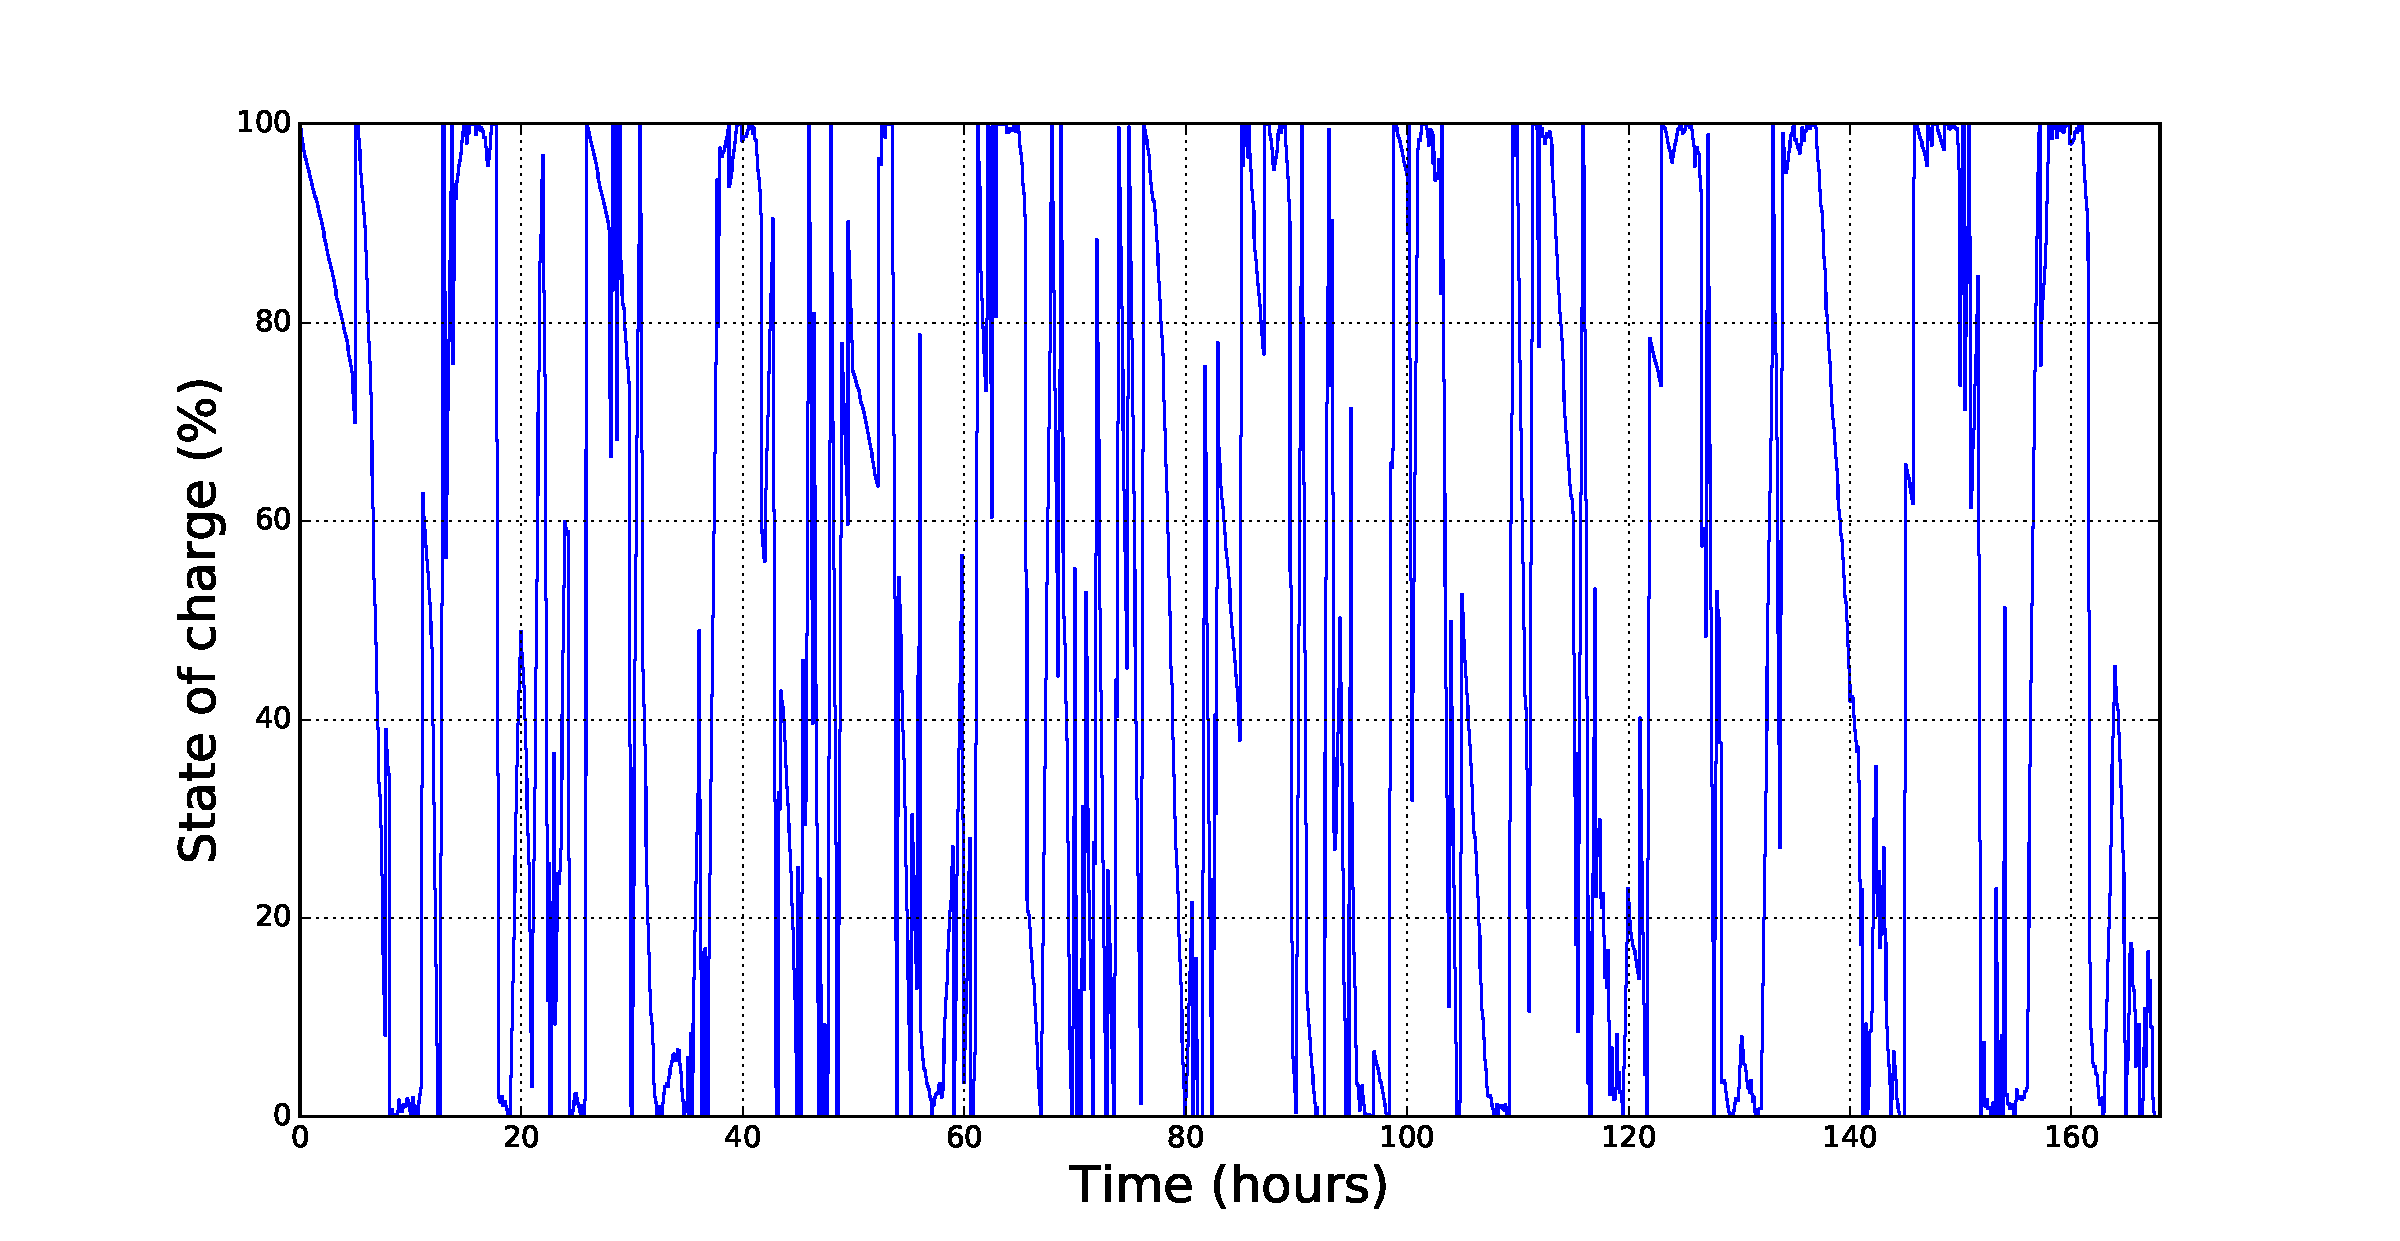
\includegraphics[width=4in]
{Figures/Plots/fullproblem_stoch/soc_fp_st.pdf} \caption{Trajectory of the state of charge of battery}\label{soc_fp_st}\end{center}
\end{figure}

\subsubsection{Upper Bound from Mean Value Problem}
\begin{figure}[h!]
\begin{center}
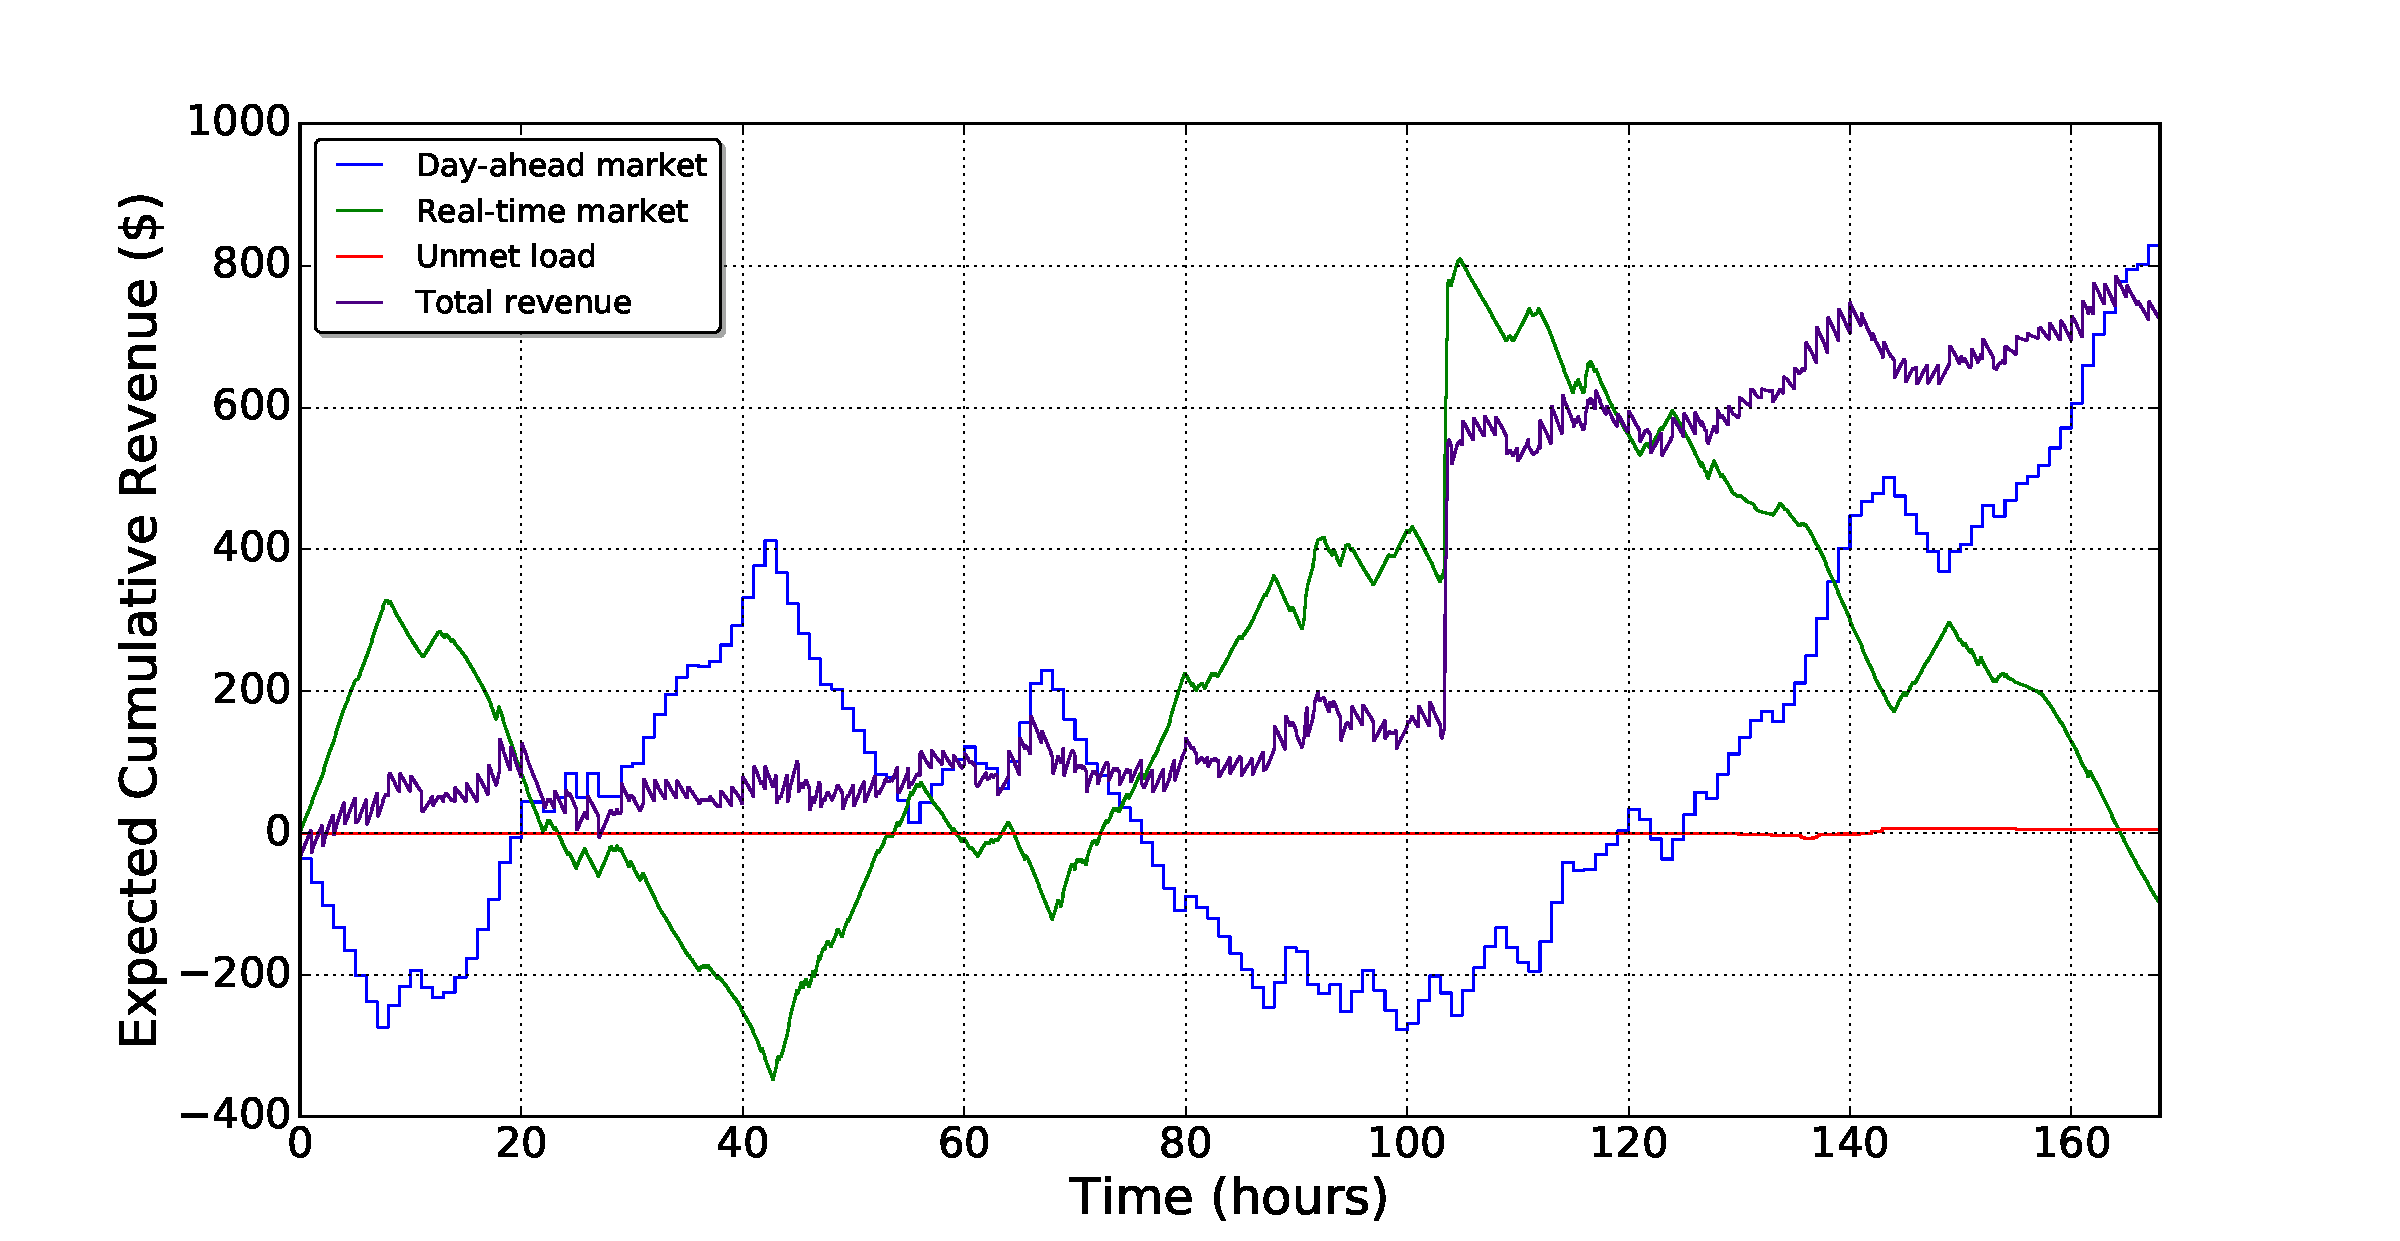
\includegraphics[width=4in]{Figures/Plots/fullproblem_det/cumulative_rev_fp_dt.pdf} \caption{Trajectory of cumulative revenues}\label{cumulative_rev_fp_dt}\end{center}
\end{figure}
\begin{figure}[h!]
\begin{center}
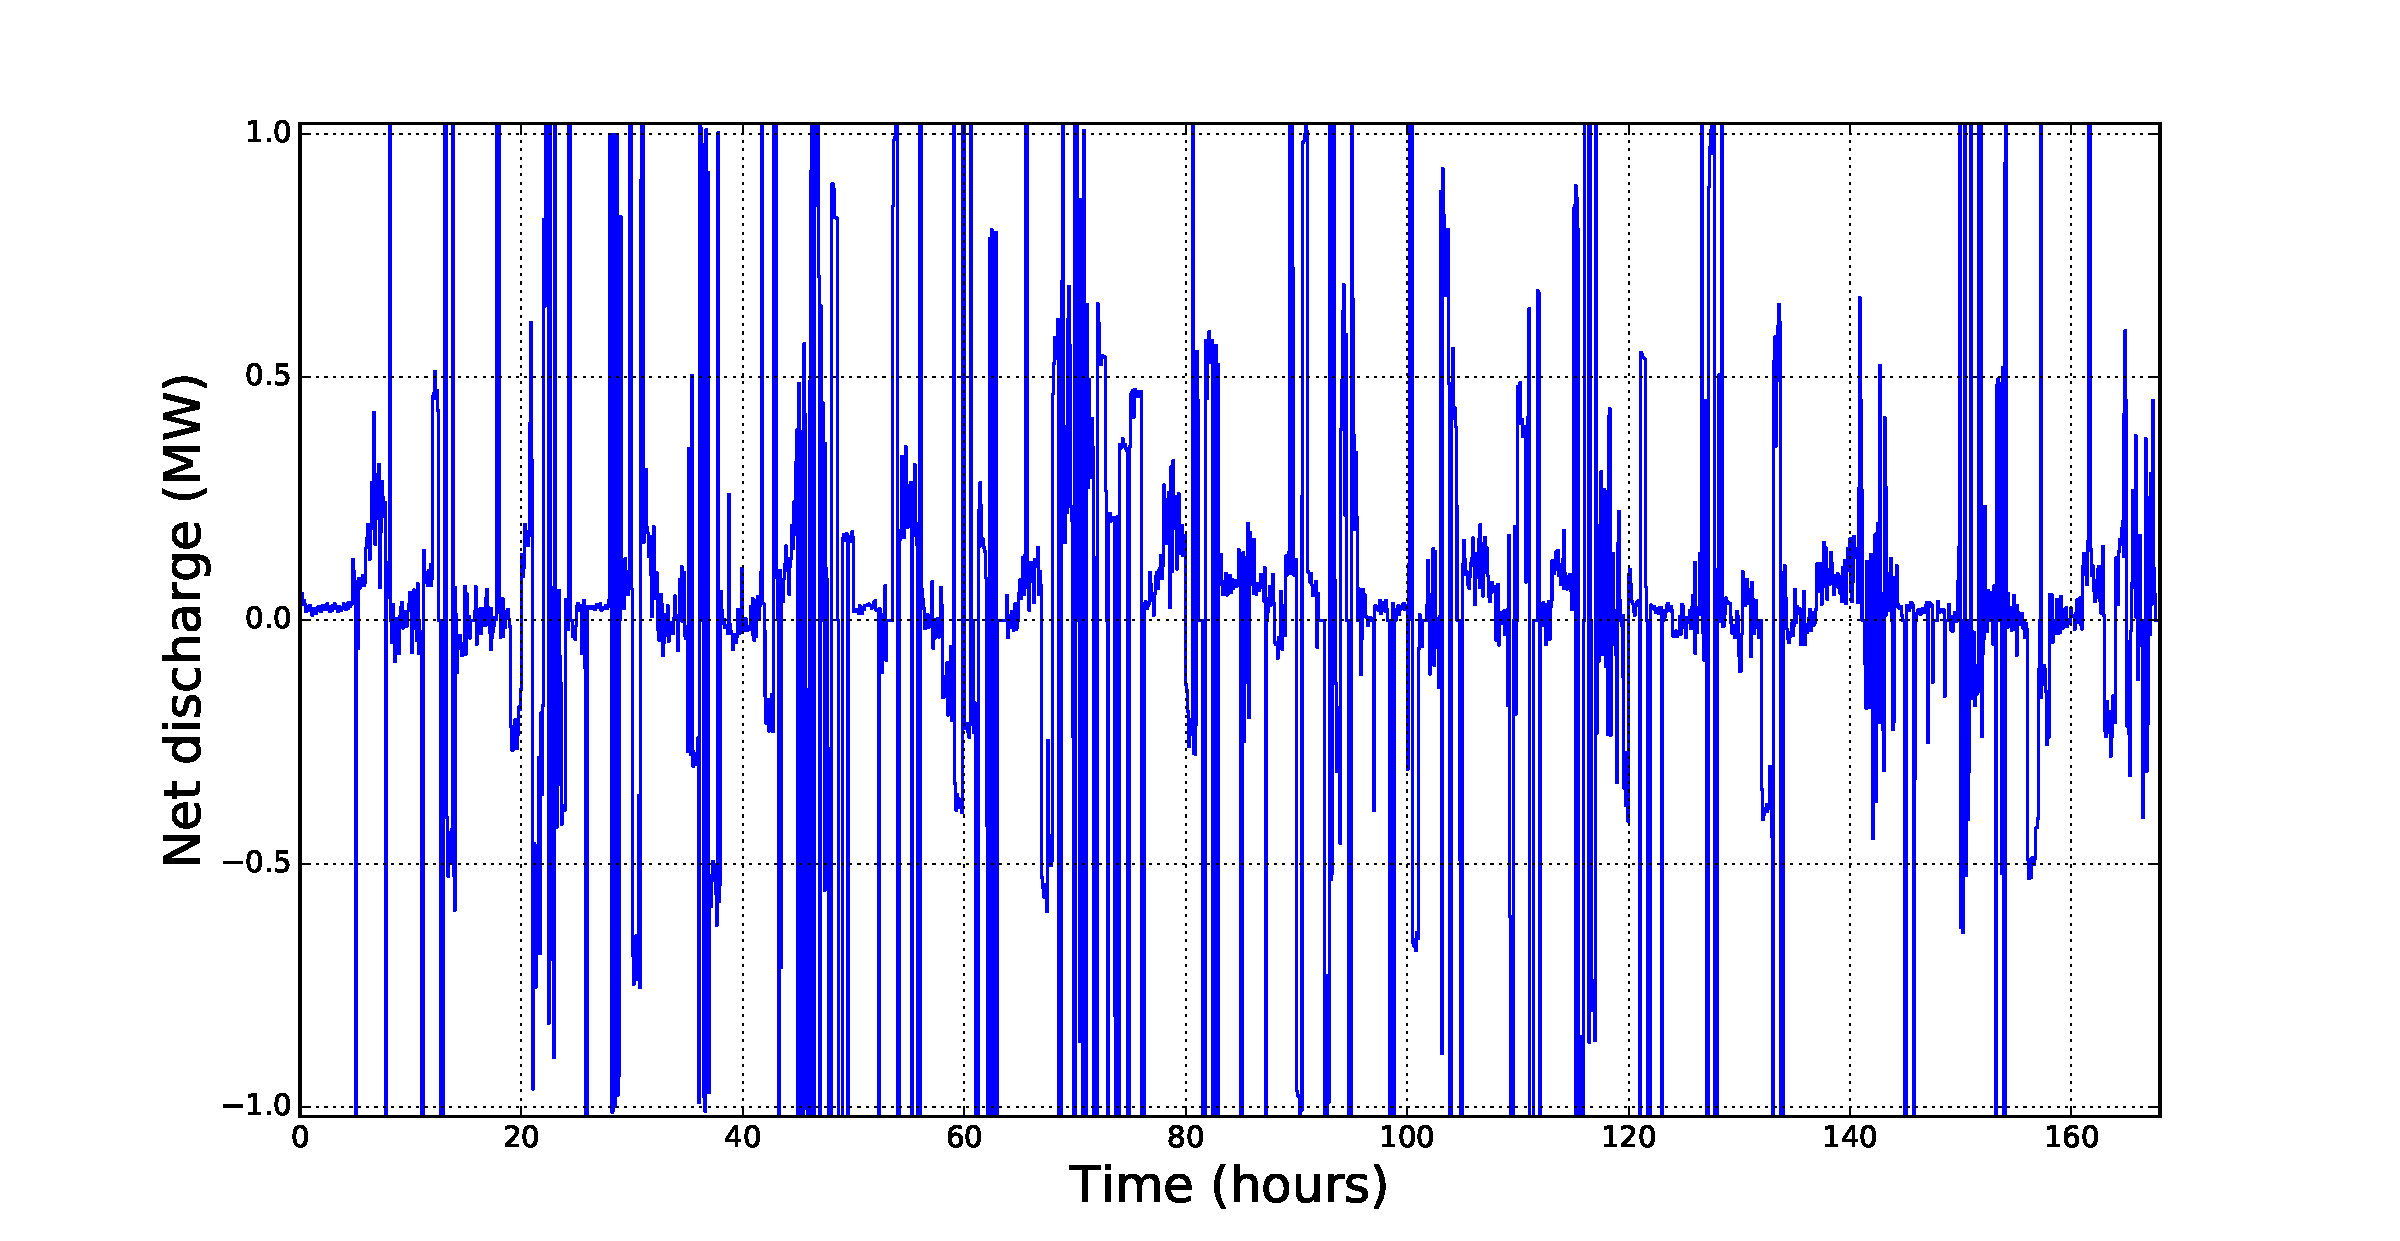
\includegraphics[width=4in]{Figures/Plots/fullproblem_det/netpower_fp_dt.pdf} \caption{Net battery discharge}\label{netpower_fp_dt}\end{center}
\end{figure}
\begin{figure}[h!]
\begin{center}
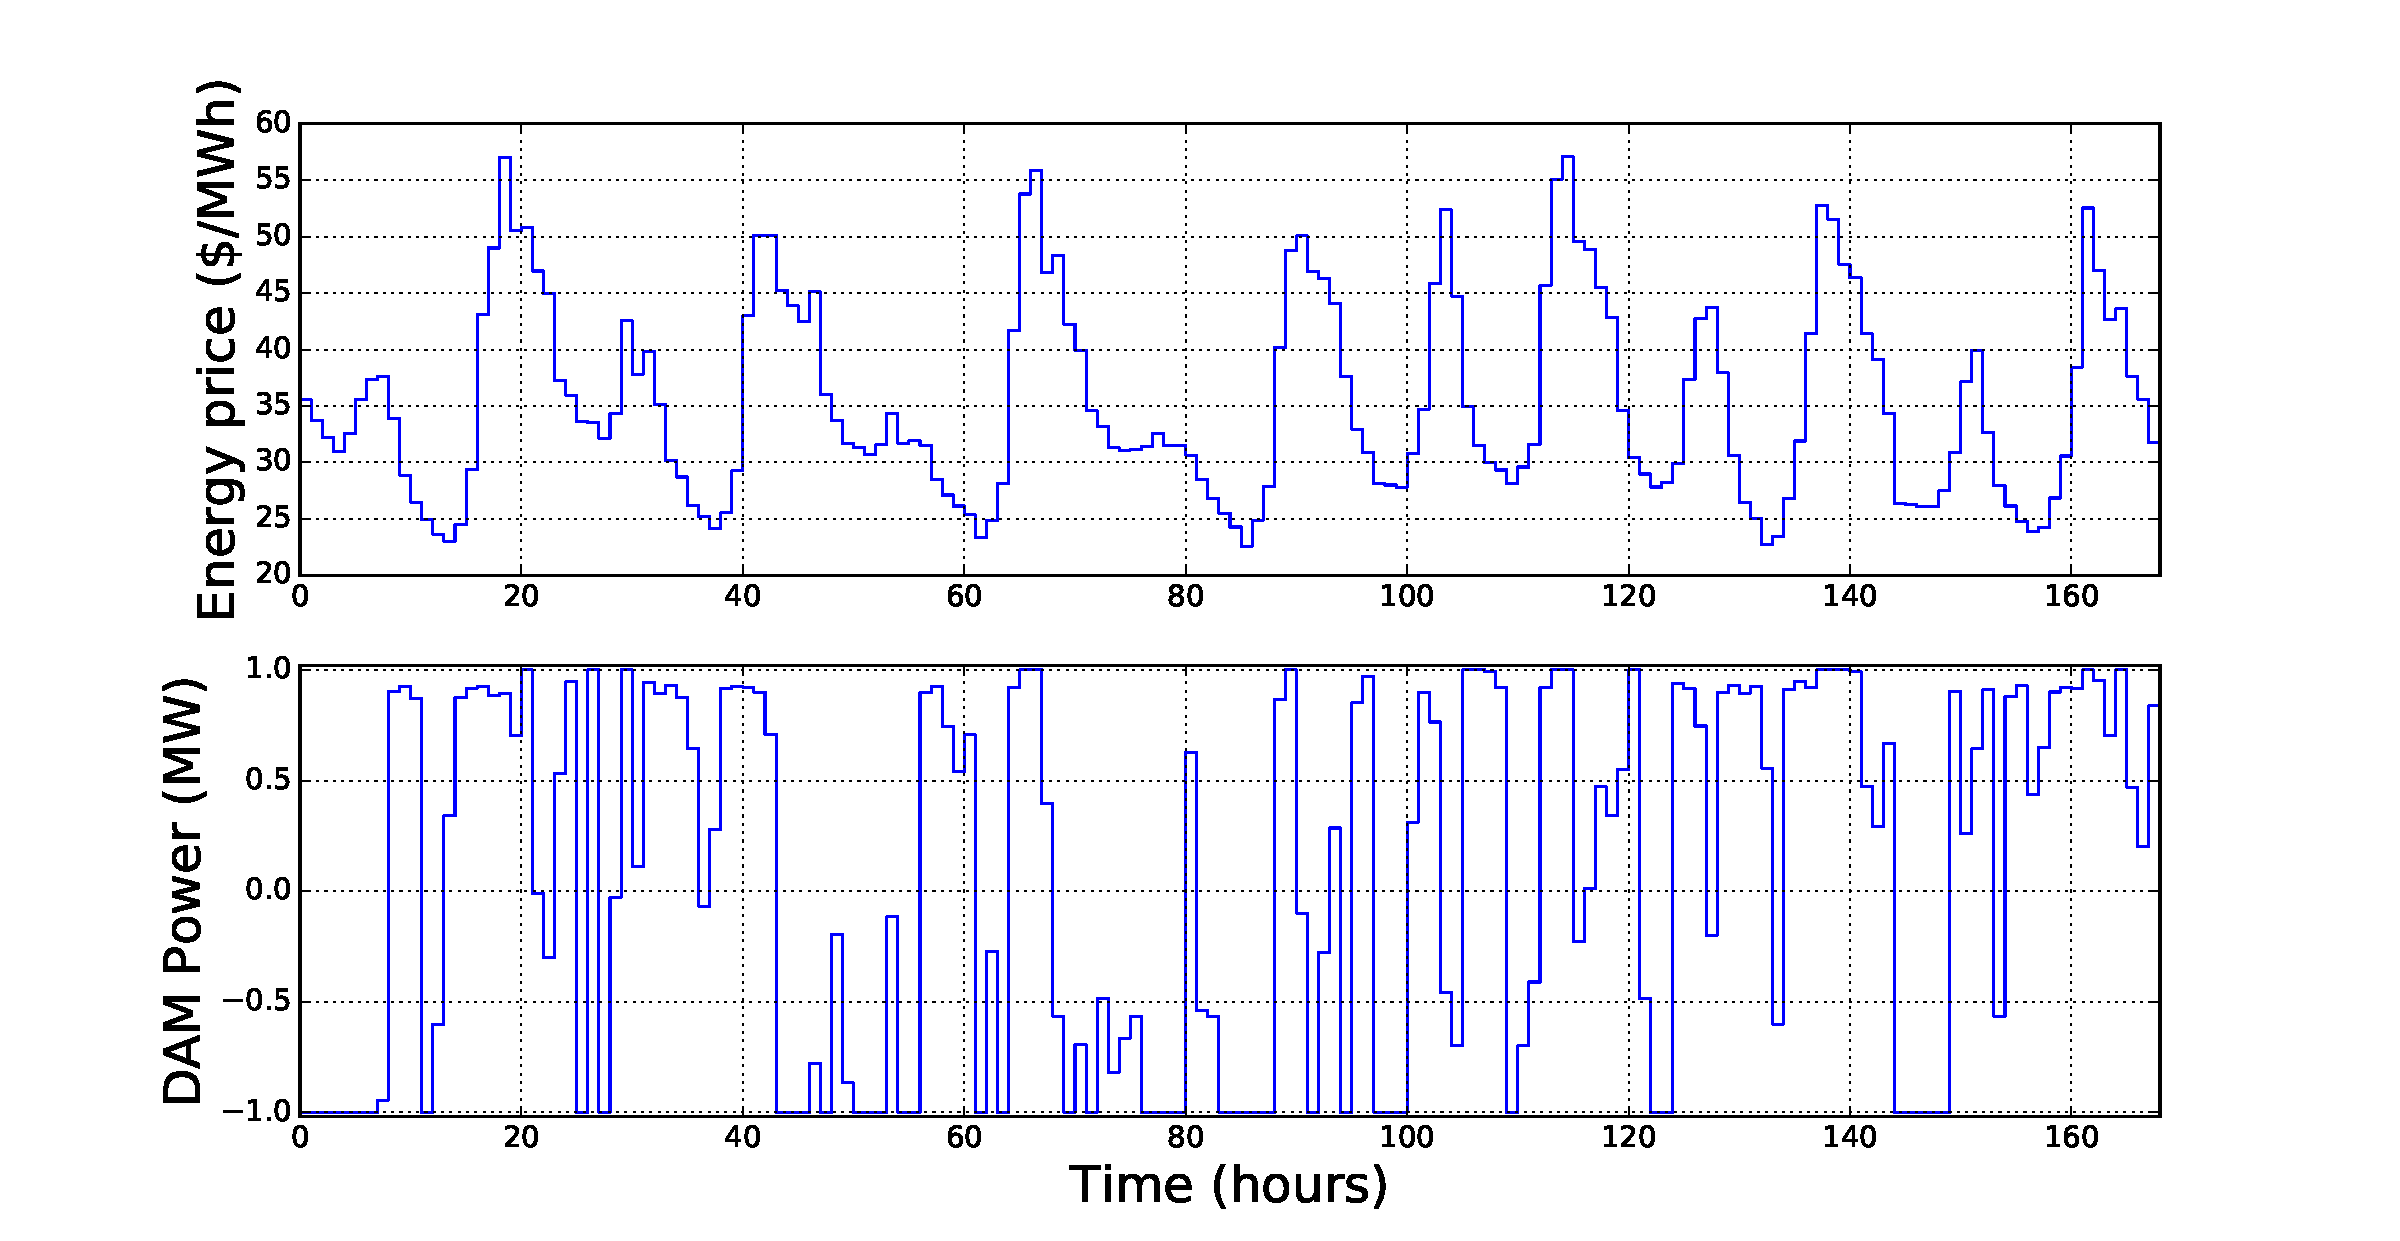
\includegraphics[width=4in]{Figures/Plots/fullproblem_det/Pdam_fp_dt.pdf} \caption{Energy participation policy in day-ahead market}\label{Pdam_fp_dt}\end{center}
\end{figure}
\begin{figure}[h!]
\begin{center}
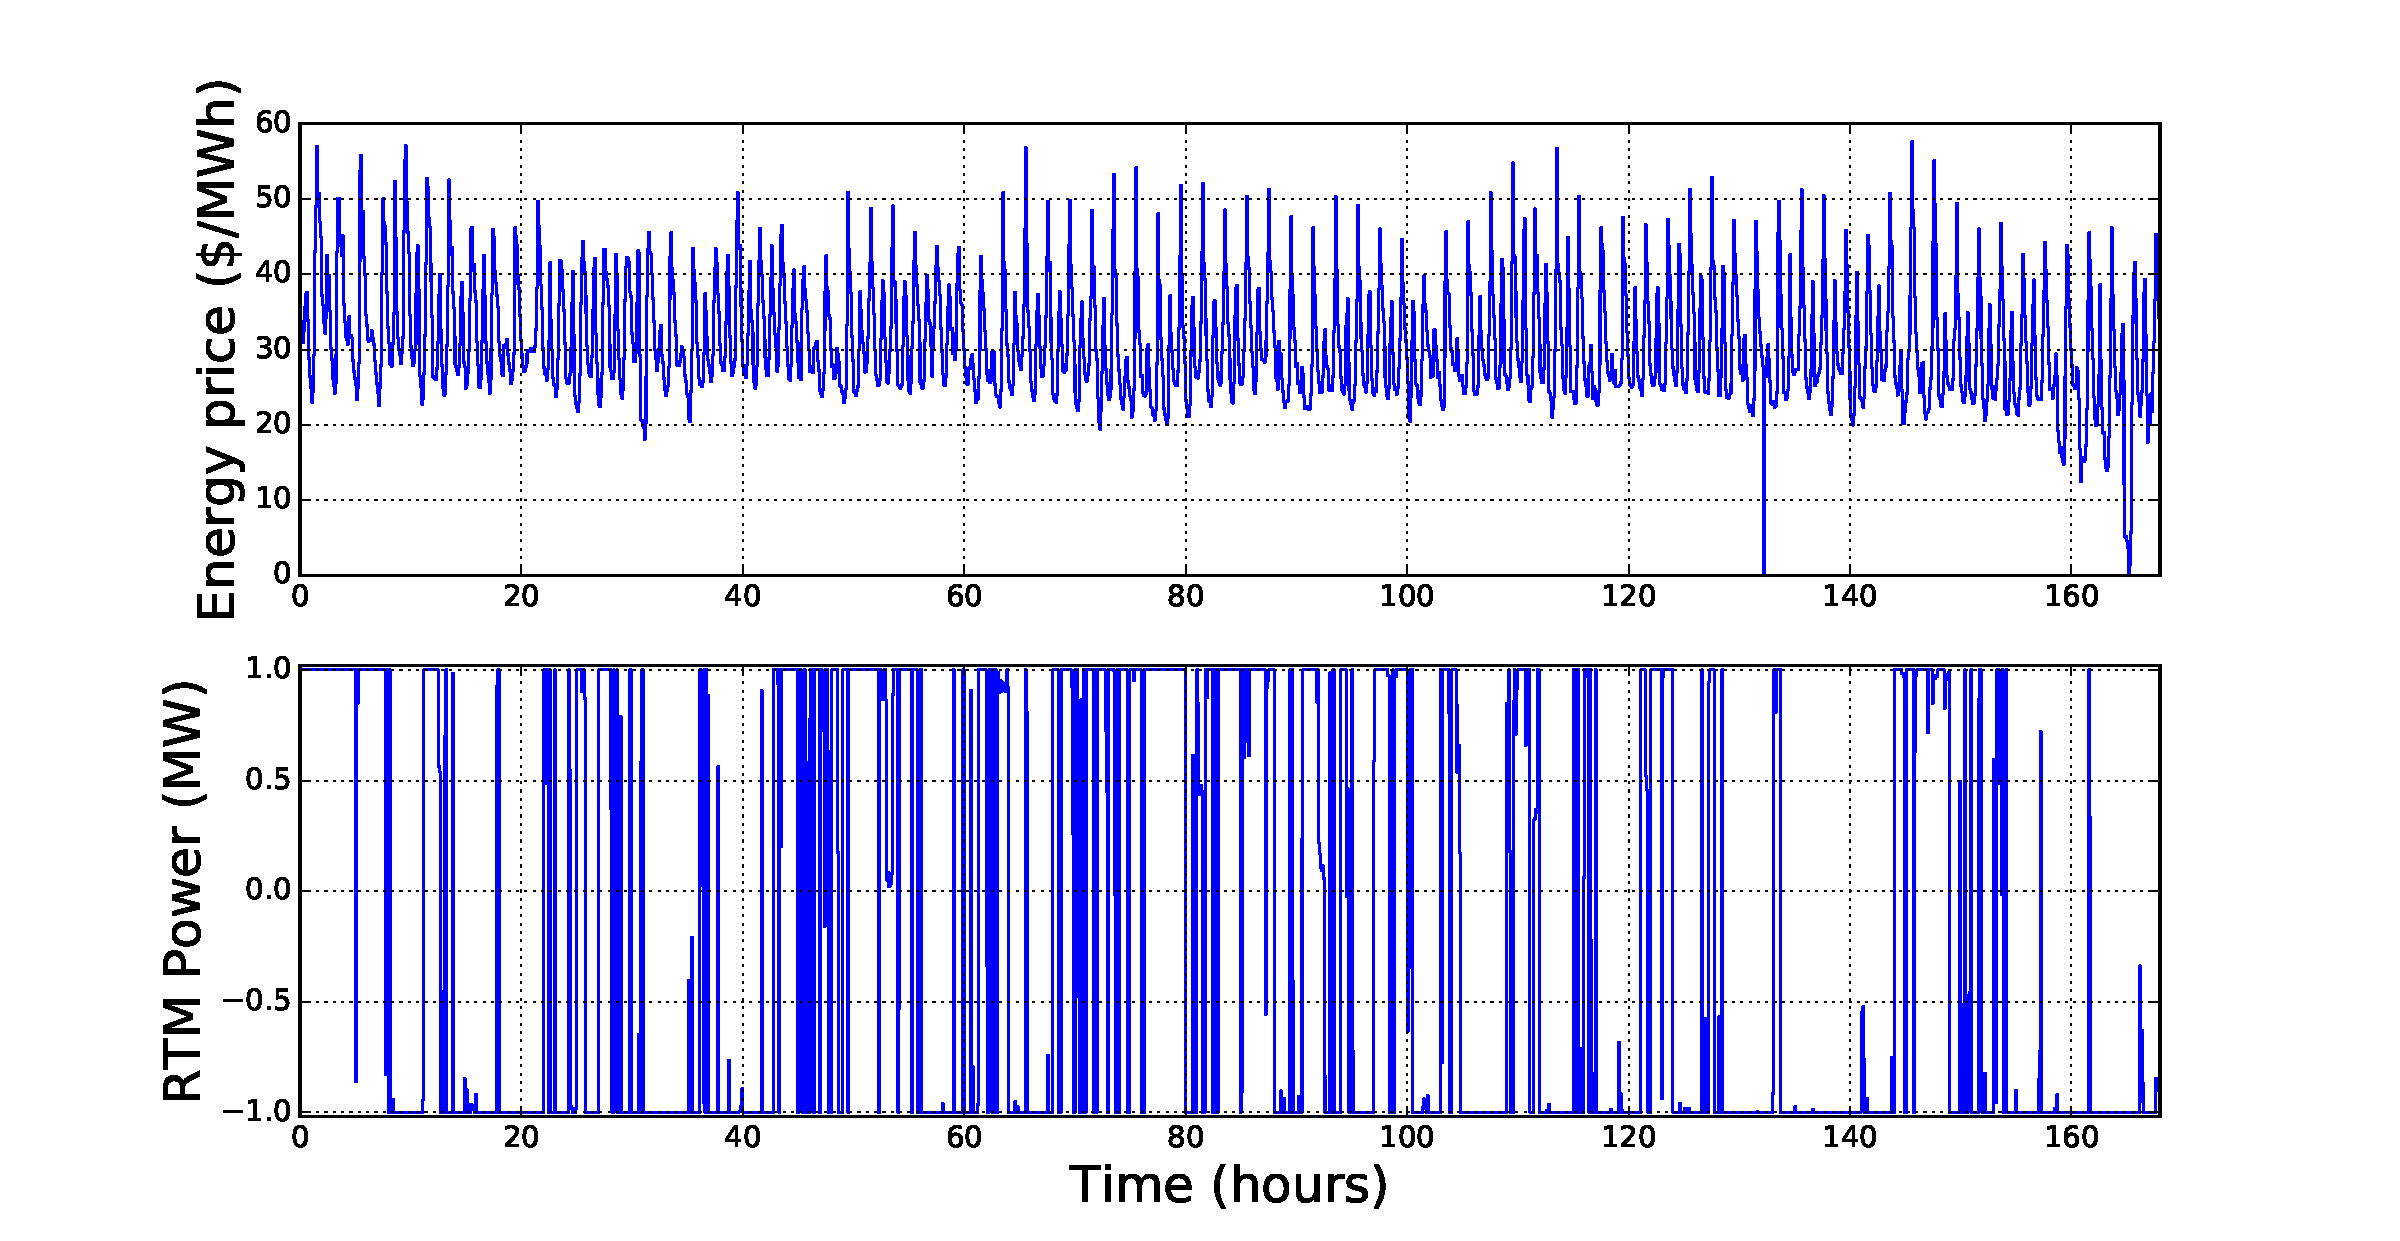
\includegraphics[width=4in]{Figures/Plots/fullproblem_det/Prtm_fp_dt.pdf} \caption{Energy participation policy in real-time market}\label{Prtm_fp_dt}\end{center}
\end{figure}
\begin{figure}[h!]
\begin{center}
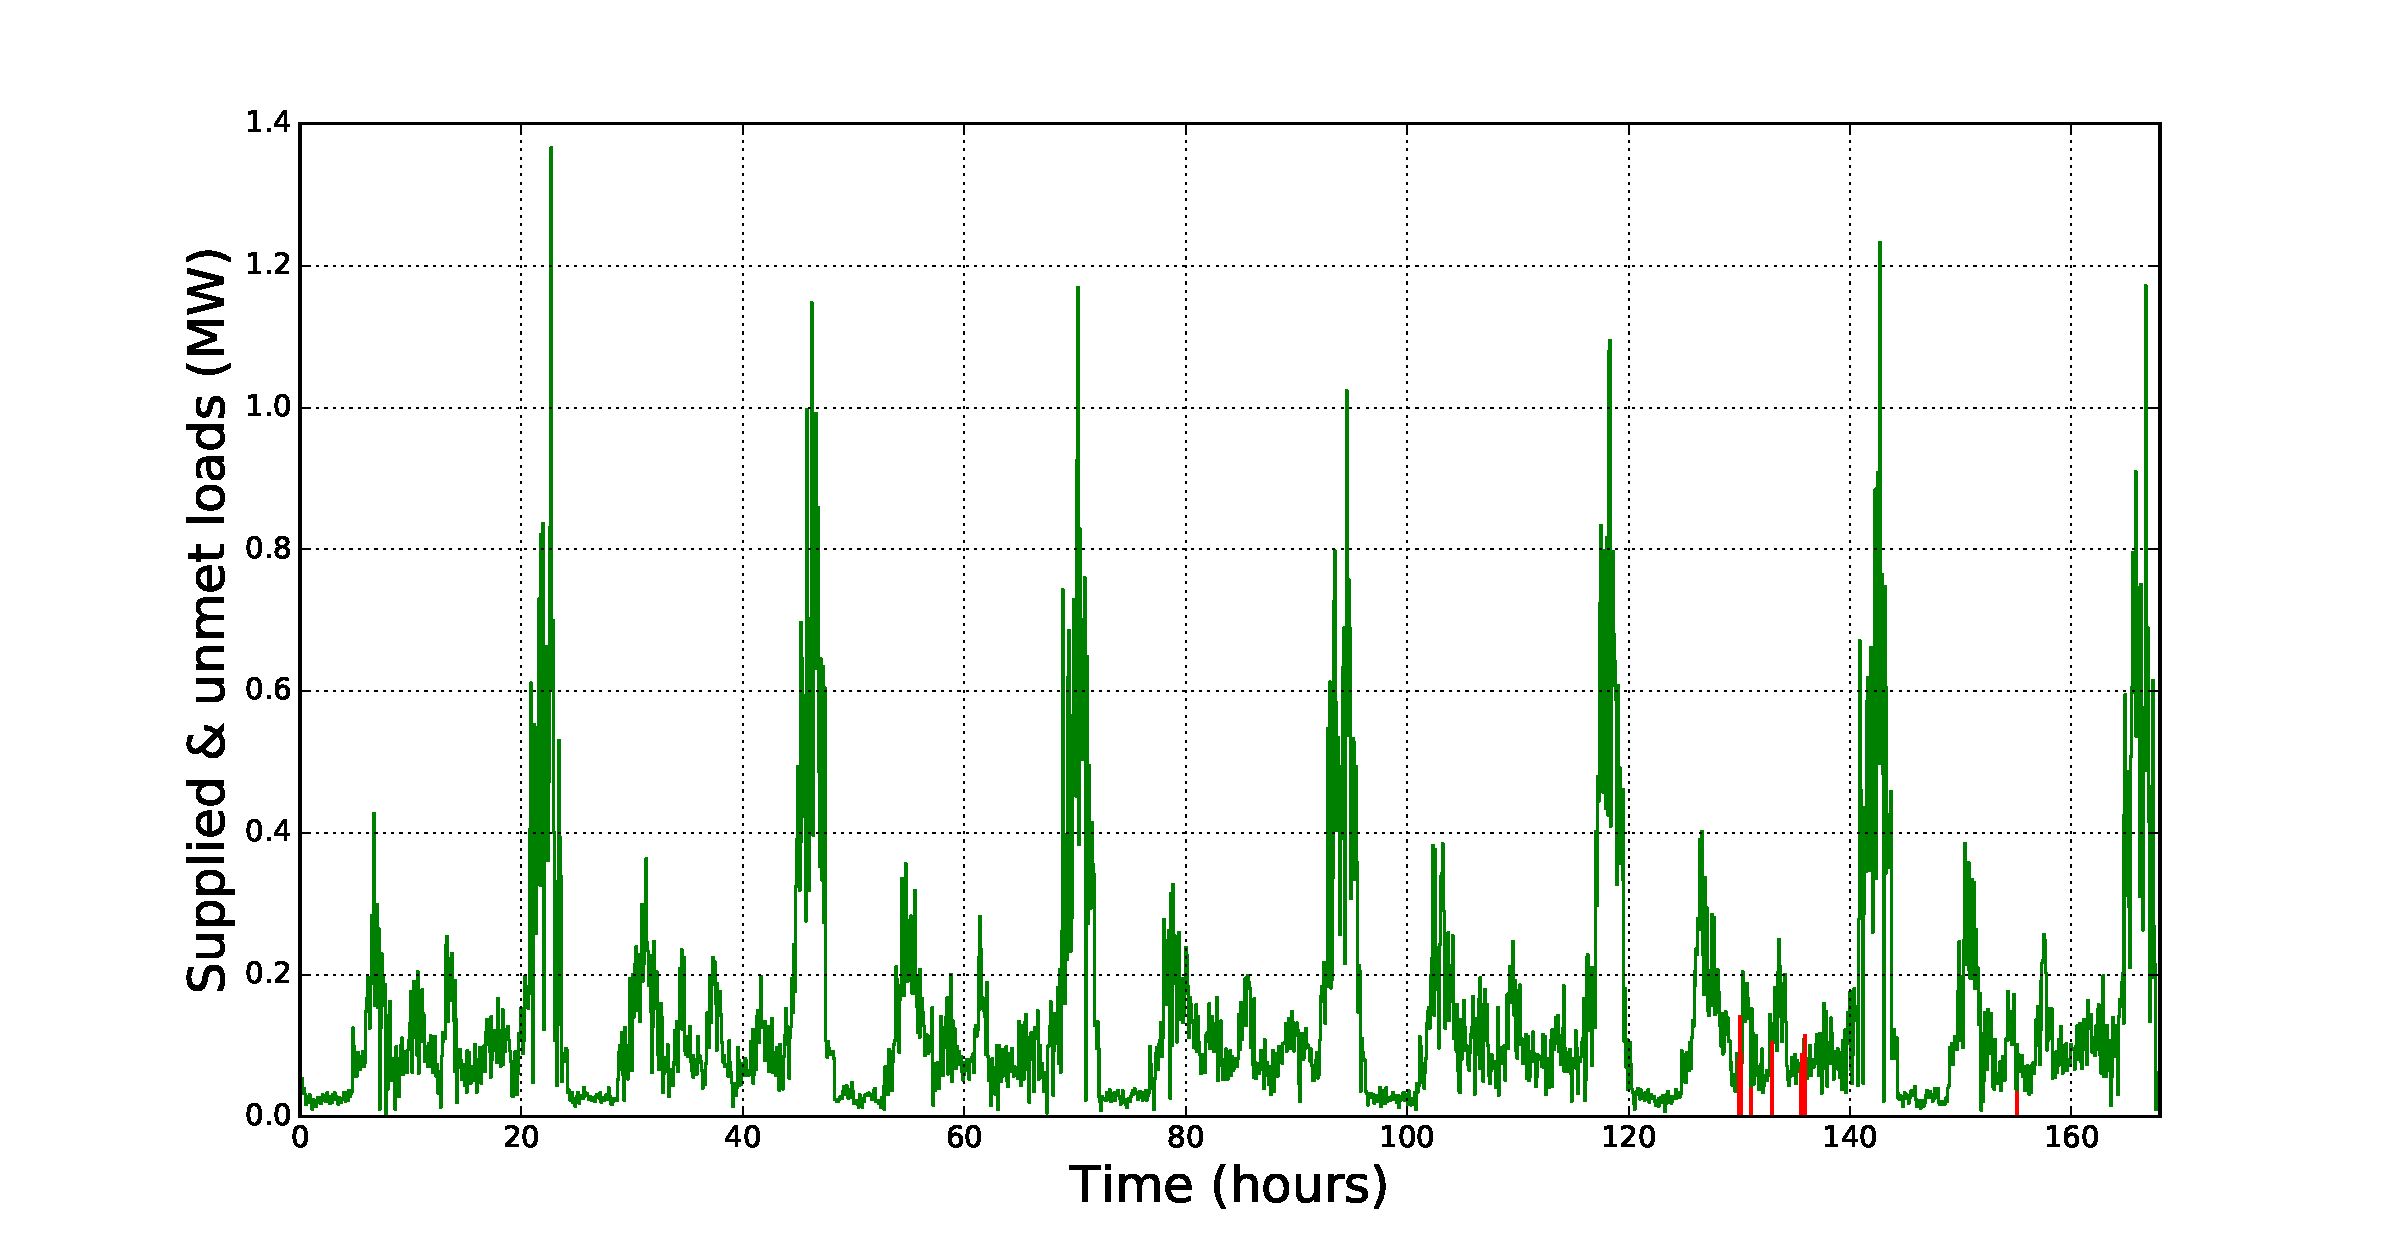
\includegraphics[width=4in]
{Figures/Plots/fullproblem_det/supp_unmet_fp_dt.pdf} \caption{Power supplied to building and unmet load}\label{supp_unmet_fp_dt}\end{center}
\end{figure}
\begin{figure}[h!]
\begin{center}
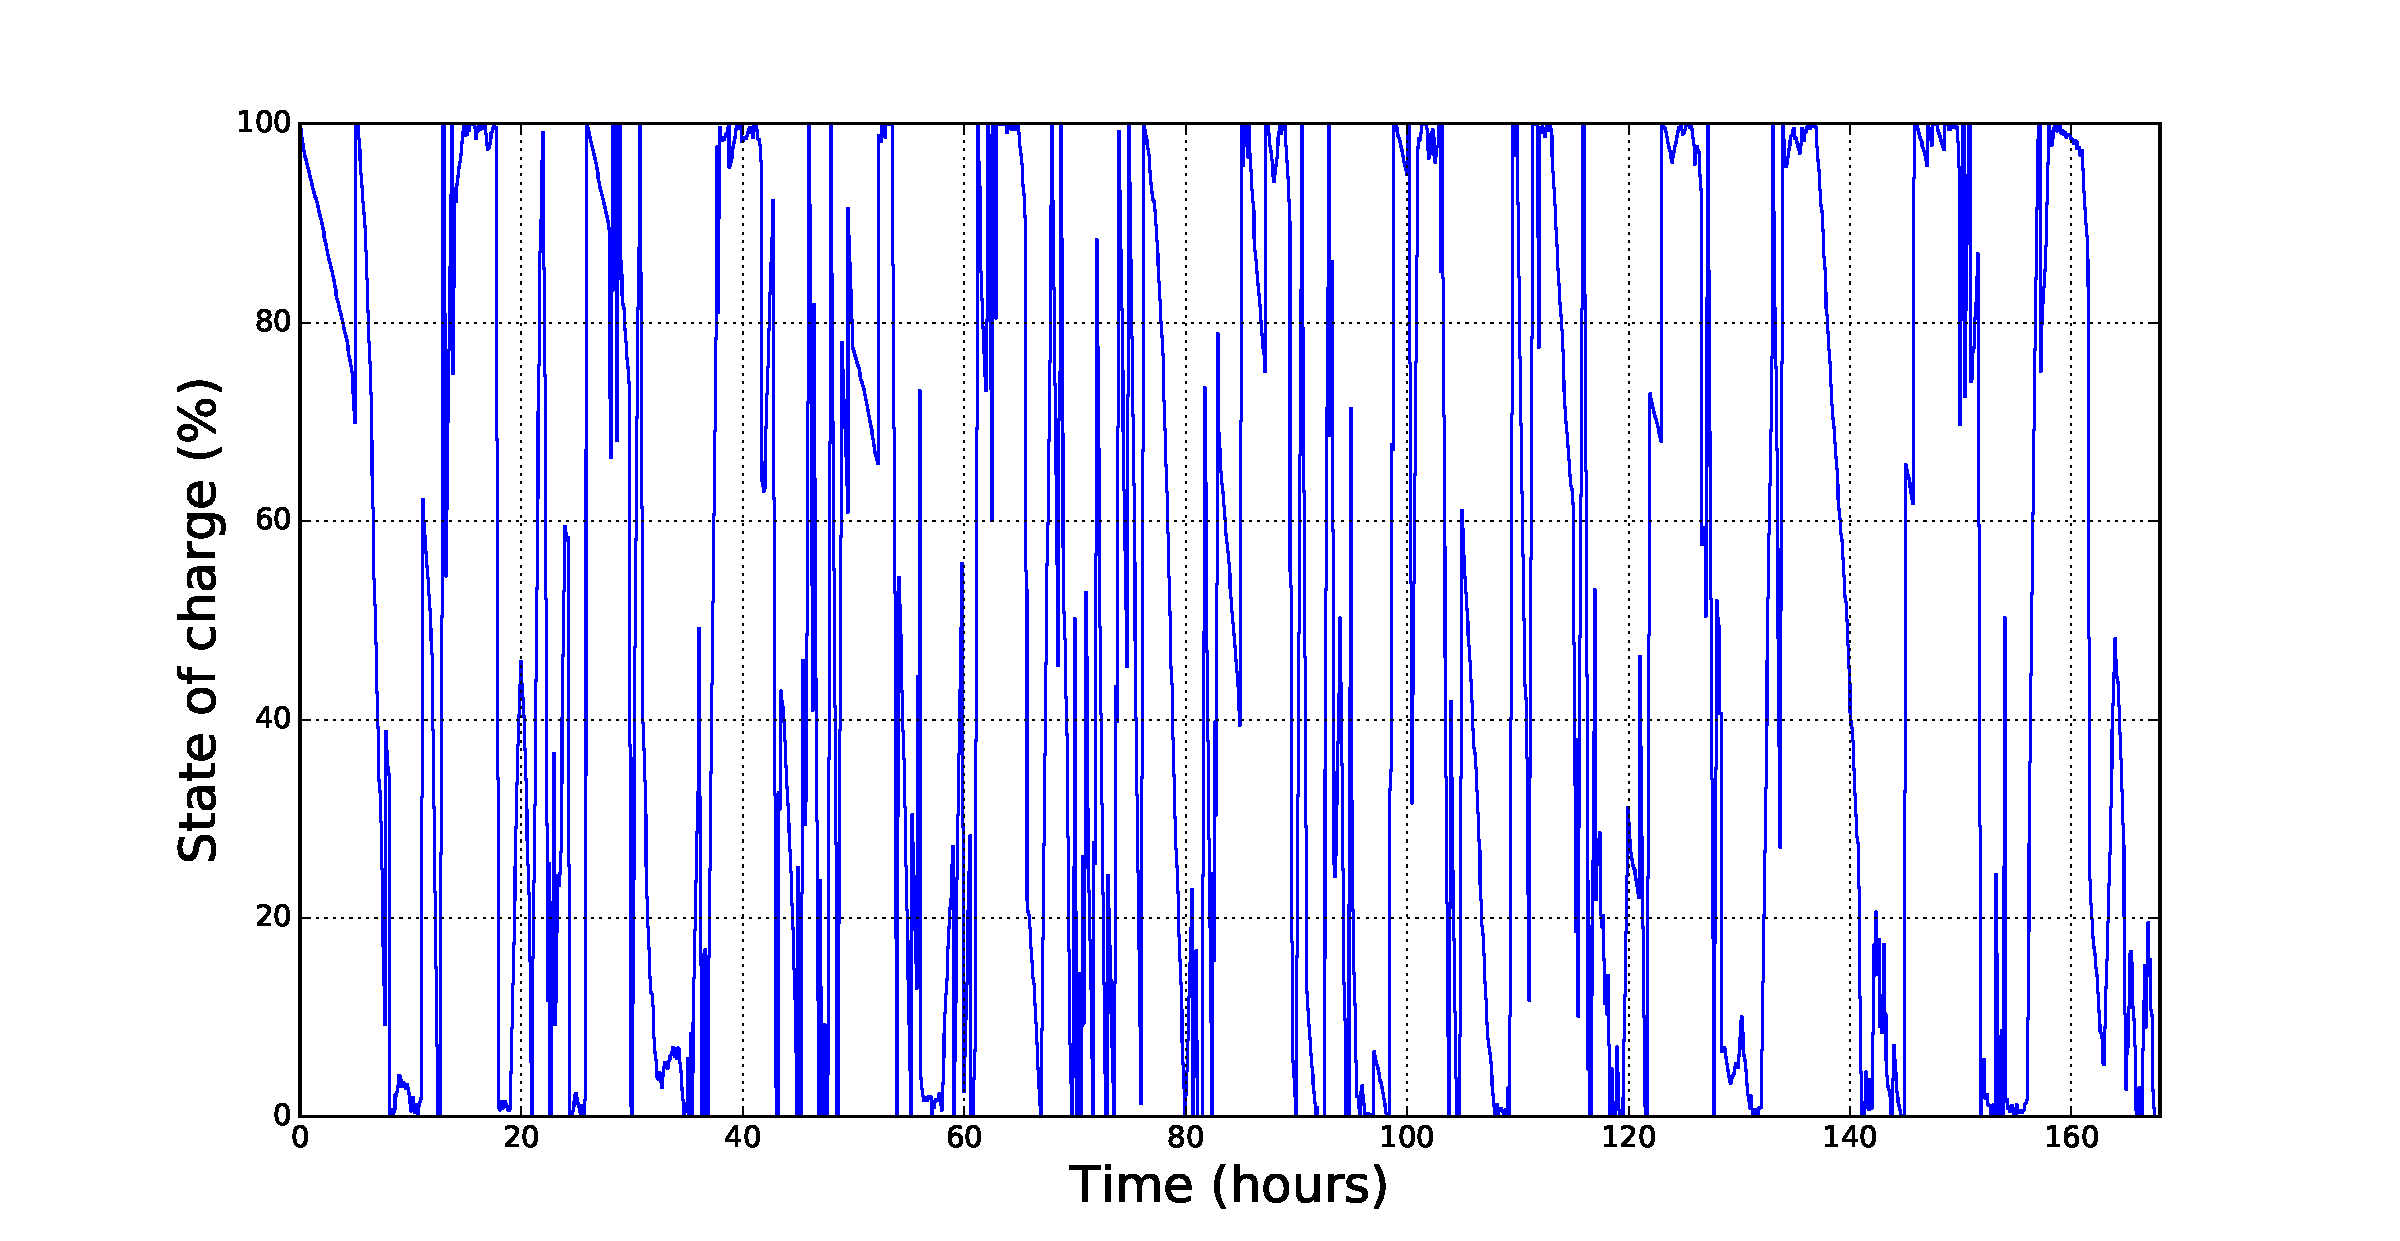
\includegraphics[width=4in]
{Figures/Plots/fullproblem_det/soc_fp_dt.pdf} \caption{Trajectory of the state of charge of battery}\label{soc_fp_dt}\end{center}
\end{figure}


\subsubsection{Estimating Bounds with Perfect Information}
\subsubsection{Estimating Bounds with Two-Stage 	Approximation: Restriction}
\subsection{Receding Horizon Heuristic}
We sample 50 paths upto next 24 hours horizon 
\subsection{Stochastic Dual Dynamic Programming}
\section{Conclusions}
\section{Future Work}
\subsection{Price Uncertainty}
\subsection{Three Layer Markets}



\bibliography{cs719}

\end{document}
